% Chapter-level section inserted immediately before the conclusion of
% chapterB.tex.

\section{The linearising coordinate in the complex plane}
\label{sec:koenigsvisual}

The analysis above has treated the Koenigs function $\psi_r$ chiefly through
the single value $A(p)=2\psi_{2p}(1/2)$ and its consequences for the branching
process. In the complex plane the same function can be read as a coordinate,
and its geometry locates that scalar within the larger analytic object from
which it comes. The figures are direct exports from the accompanying interactive
program.\footnote{\texttt{koenigs\_explorer.html}, supplied with the chapter
files. The captions record the parameter values used for the exports.}

\subsection{Basin geometry and orbit capture}

For fixed $r$, the iteration-limit representation
\[
\psi_r(z)=\lim_{n\to\infty}r^{-n}f_r^{\circ n}(z)
\]
is obtained by following an orbit as it is drawn towards the origin. Its natural
domain here is the attracting basin $\{z:f_r^{\circ n}(z)\to0\}$, and this is
the limit evaluated by the program. A seed may be captured within a few steps, reach the
same fixed point only after a long irregular transient, or escape to infinity
(Figure~\ref{fig:koenigs-orbit}). The first two behaviours therefore belong to
the same basin, however different their transients appear; the third does not.
Passing from these individual orbits to the set of all captured seeds produces
the coloured region in Figures~\ref{fig:koenigs-orbit} and
\ref{fig:koenigs-surface}, and in panels (a)--(e) of
Figure~\ref{fig:koenigs-seq}. Its boundary is the Julia set of $f_r$
\cite{Milnor2006}, which separates the attracting basin from the escaping
dynamics; the plotted boundary is therefore dynamical.

\begin{figure}[H]
    \centering
    \begin{subfigure}[b]{0.28\textwidth}
        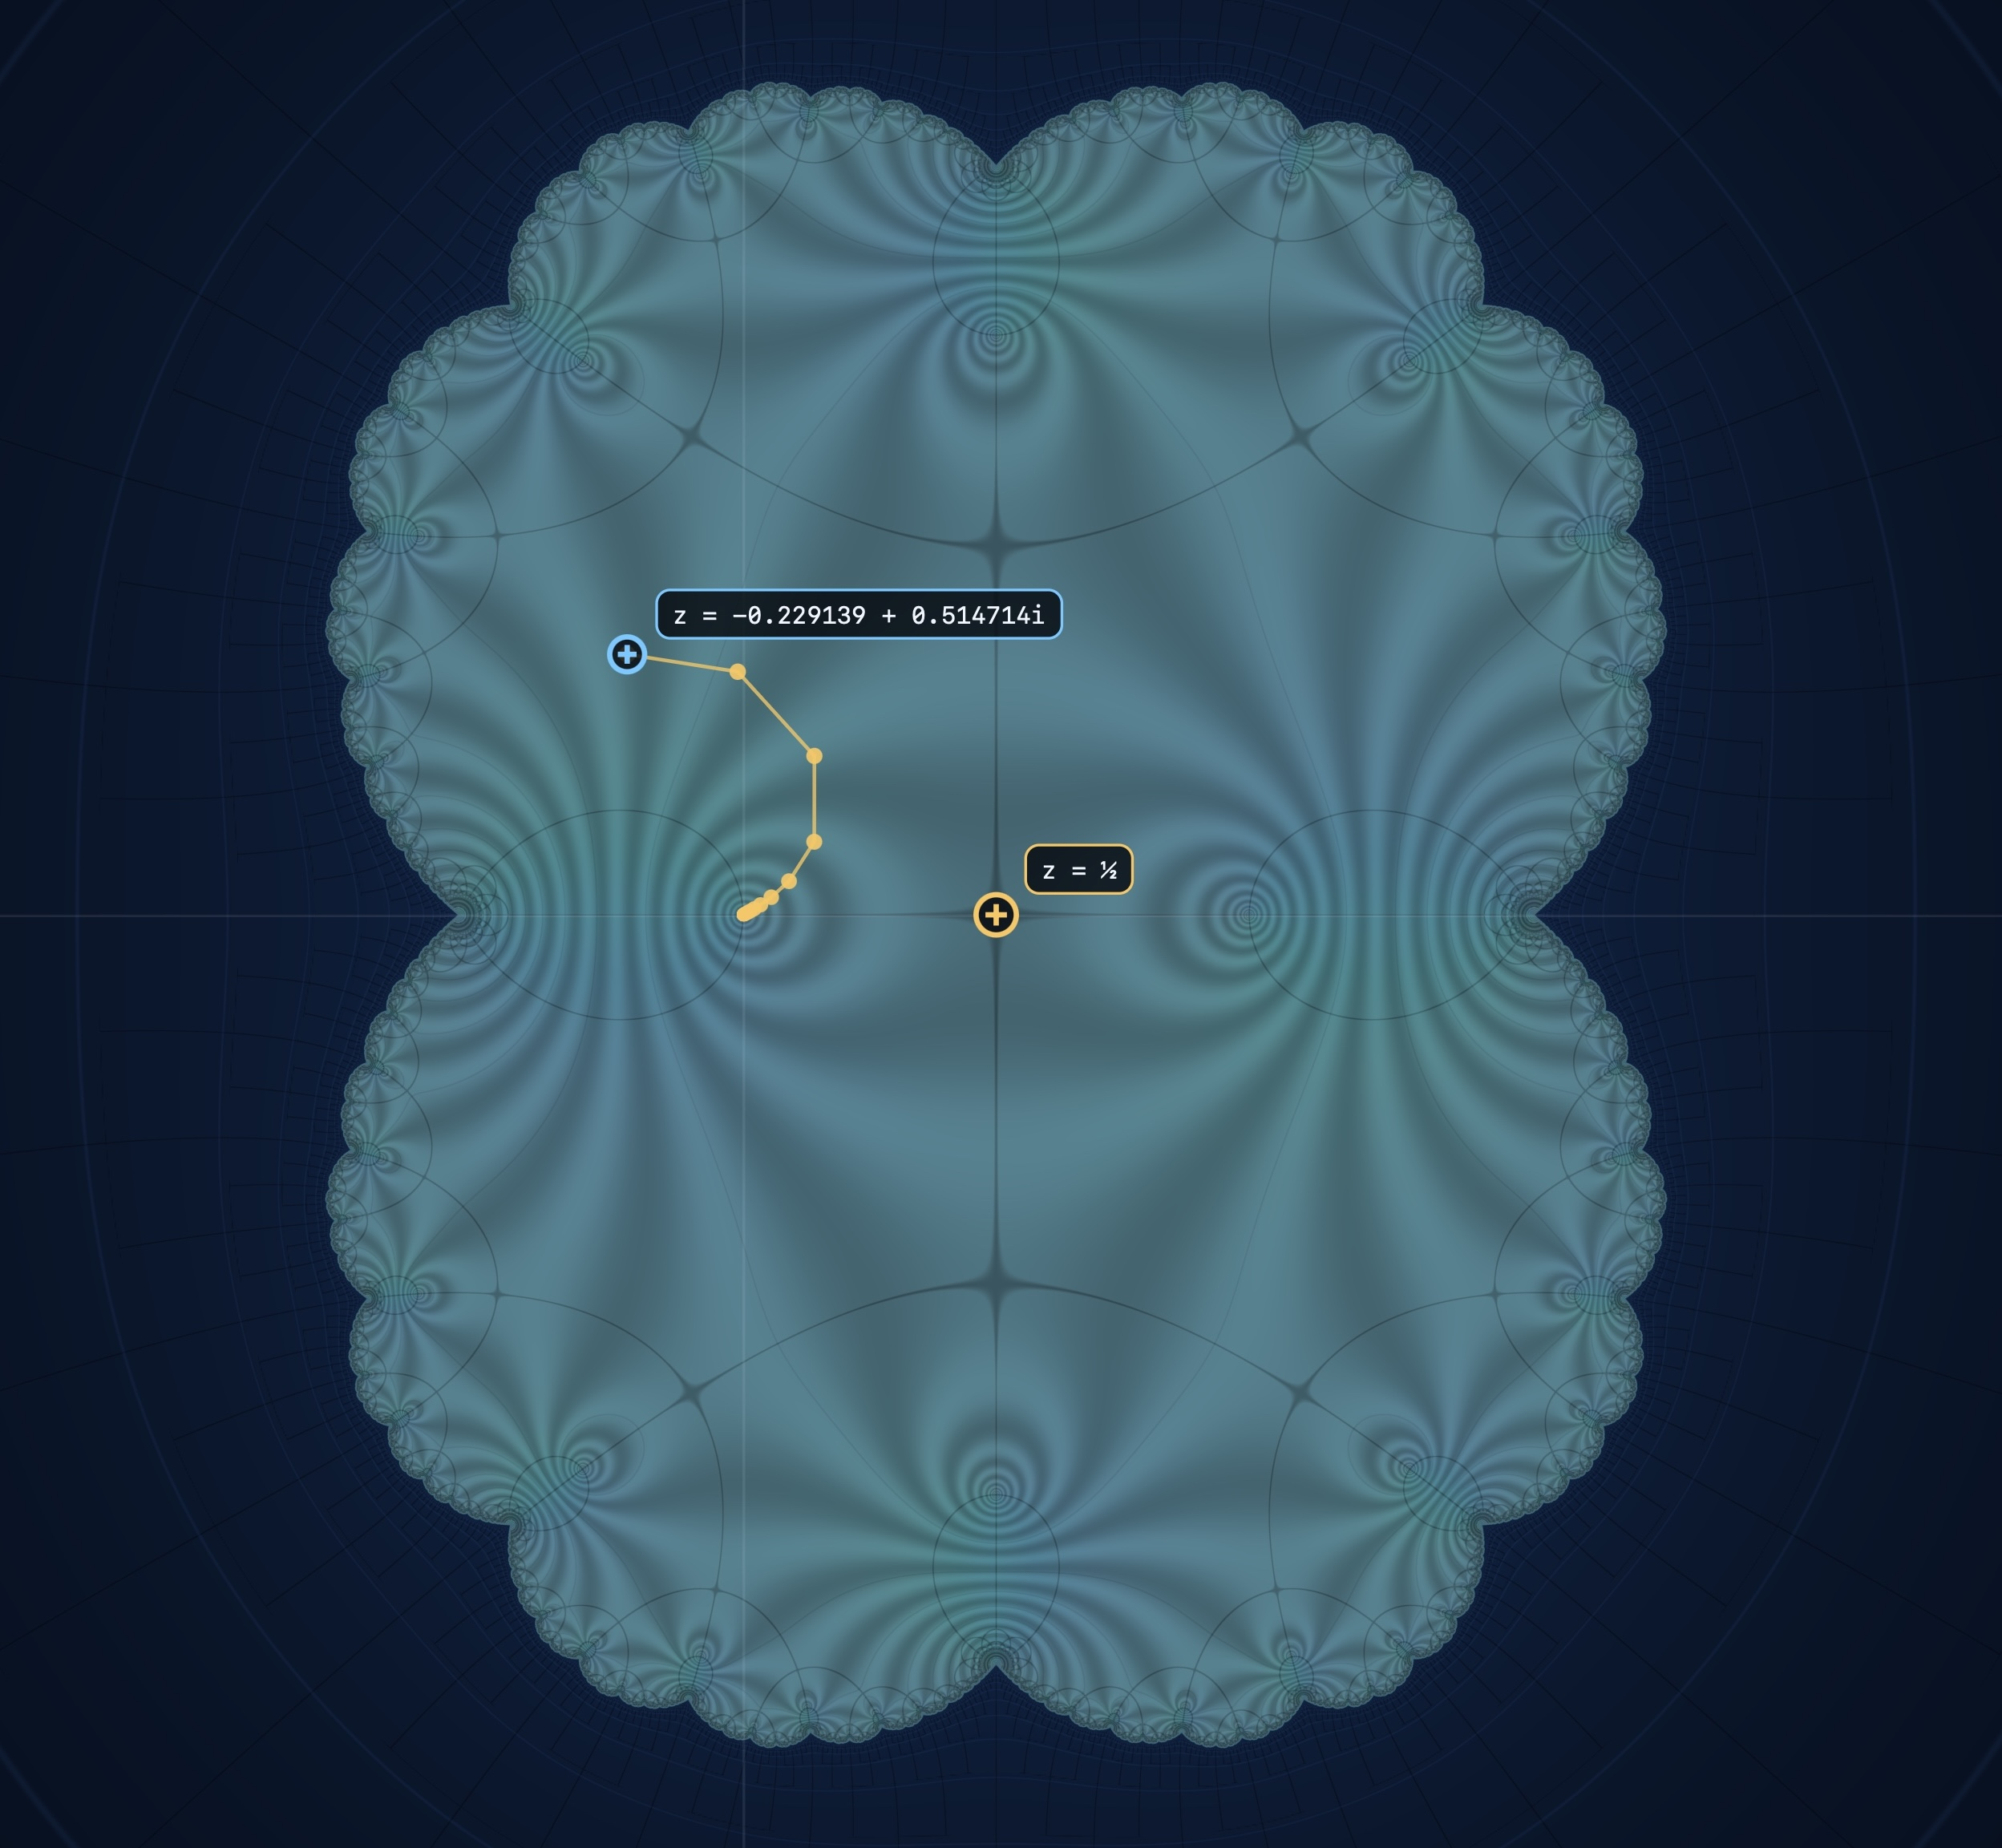
\includegraphics[width=\textwidth]{pictures/1.jpg}
        \caption{Rapid capture.}
    \end{subfigure}
    \hfill
    \begin{subfigure}[b]{0.28\textwidth}
        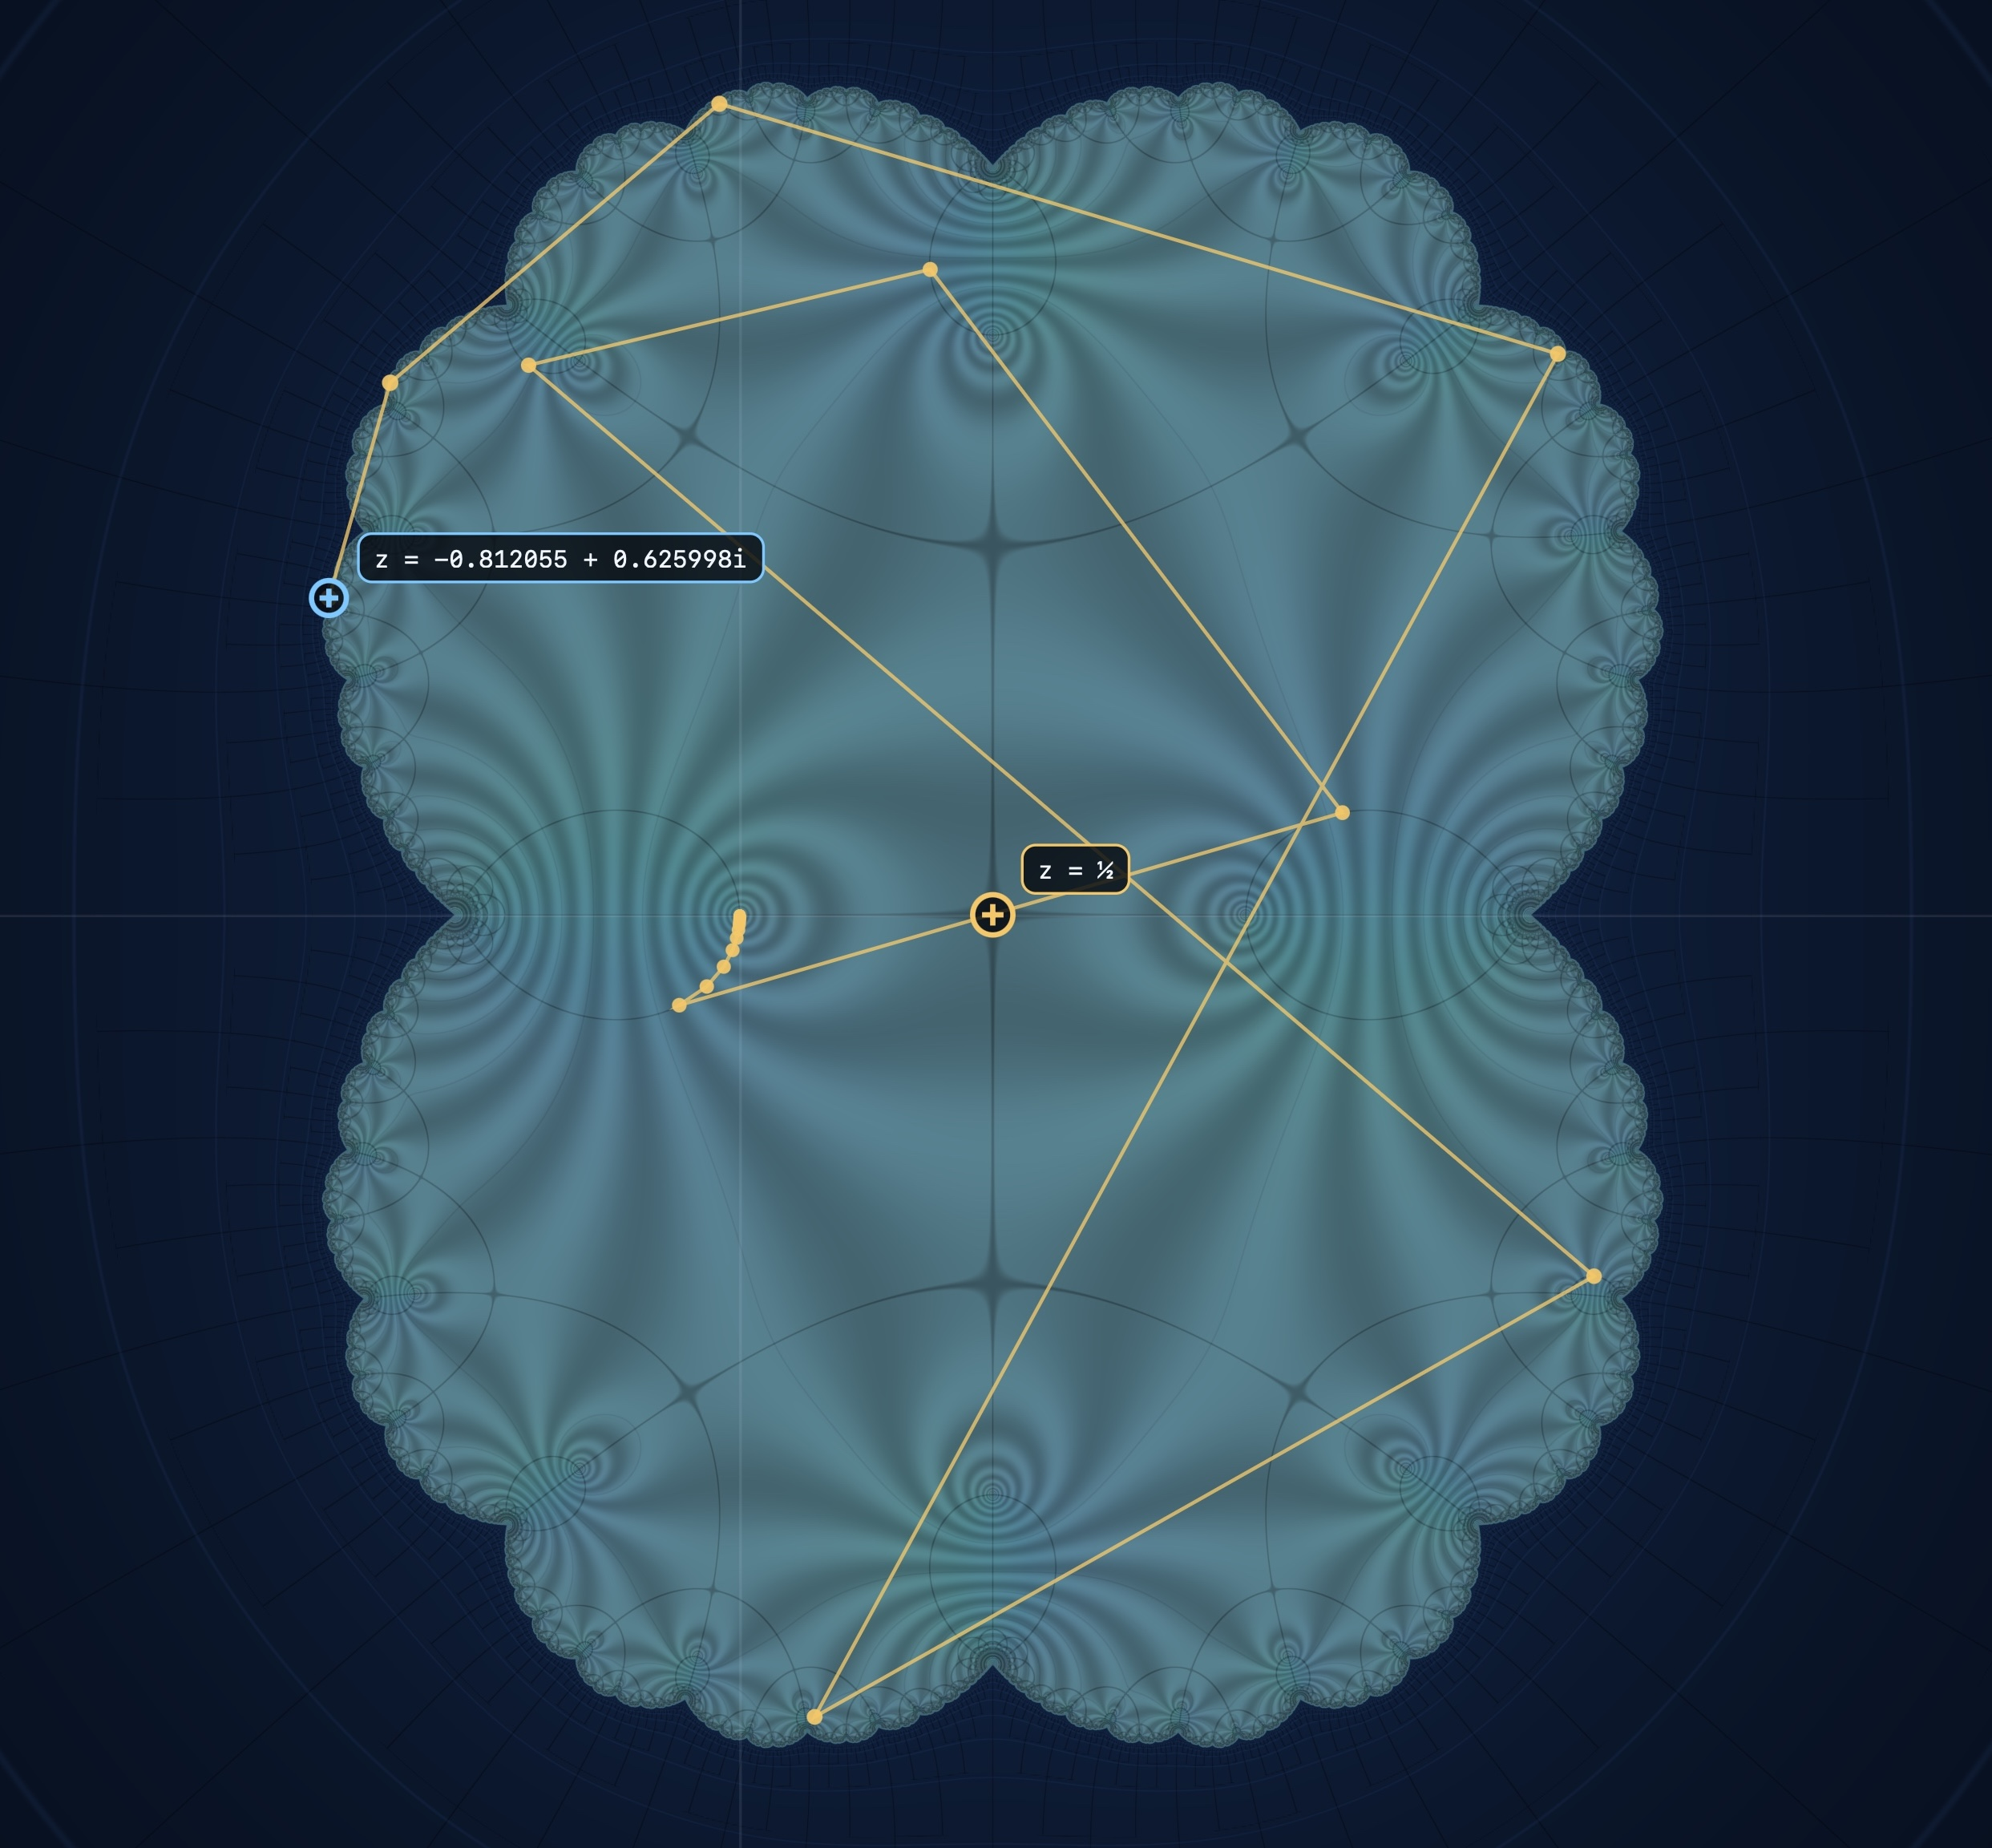
\includegraphics[width=\textwidth]{pictures/2.jpg}
        \caption{Capture after a long transient.}
    \end{subfigure}
    \hfill
    \begin{subfigure}[b]{0.28\textwidth}
        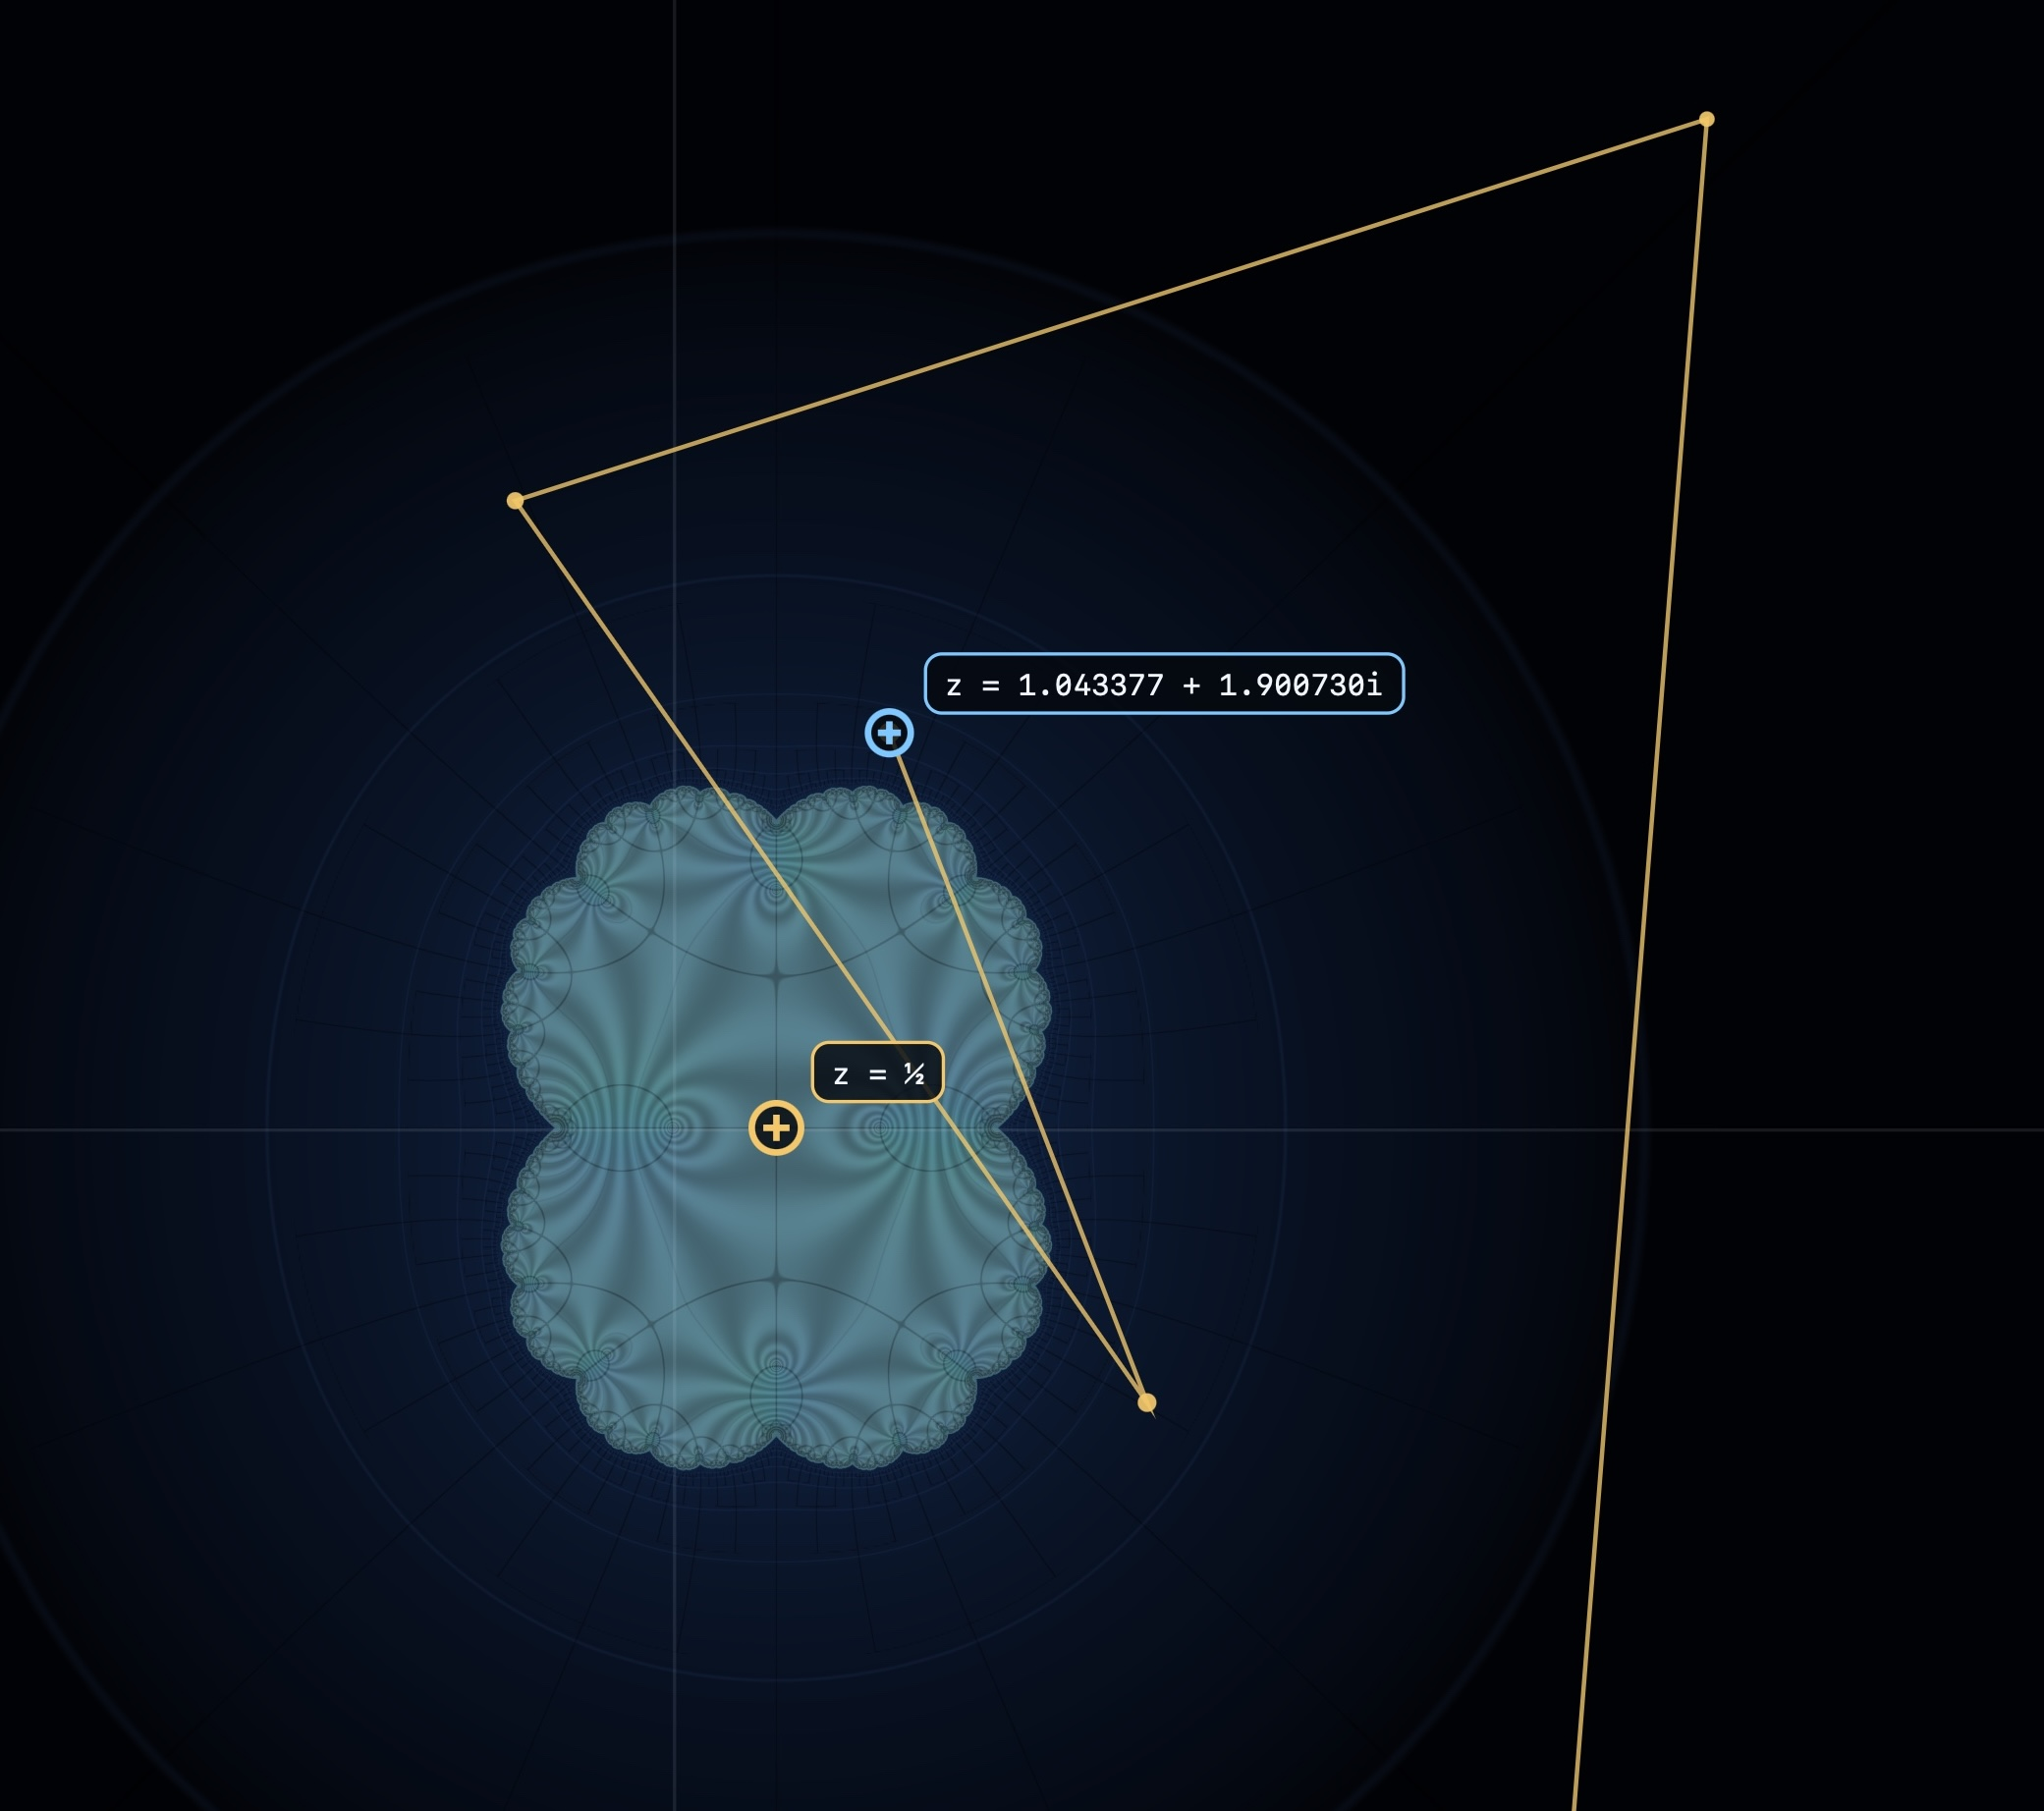
\includegraphics[width=\textwidth]{pictures/3.jpg}
        \caption{Escape to infinity.}
    \end{subfigure}

    \caption{Orbit fates for $f_r(z)=rz(1-z)$ at $r=0.64$ ($p=0.32$). The seeds
    $z=-0.229139+0.514714i$, $z=-0.812055+0.625998i$ and
    $z=1.043377+1.900730i$ in (a)--(c) give, respectively, rapid capture,
    capture after a long transient and escape. The first two therefore lie in
    the same attracting basin.}
    \label{fig:koenigs-orbit}
\end{figure}

\FloatBarrier

\subsection{The Koenigs coordinate and the constant \texorpdfstring{$A(p)$}{A(p)}}

What is drawn inside the basin is the Koenigs coordinate itself. The black
curves are the Cartesian grid of the linearised plane,
\[
\{\operatorname{Re}\psi_r=\mathrm{const}\},
\qquad
\{\operatorname{Im}\psi_r=\mathrm{const}\},
\]
pulled back through $\psi_r$ into the nonlinear $z$-plane. In the coordinate
$y=\psi_r(z)$ this grid is regular and uniform; the figures record its distortion
when expressed in $z$. The functional equation
\[
\psi_r\bigl(f_r(z)\bigr)=r\psi_r(z)
\]
then accounts for the nested geometry. Multiplication by $r$ preserves the form
of the linearised grid while rescaling it and, when $r$ is complex, rotating it.
Pulled back to the basin, this scaling law produces progressively smaller copies
towards the attracting fixed point, with each cell recurring inside the next.
The nested detail is therefore the functional equation made visible. The
attracting Koenigs coordinate defined here has the basin as its natural domain;
the dark exterior is instead shaded by escape rate.

\begin{figure}[!b]
    \centering
    \begin{subfigure}[b]{0.57\textwidth}
        \centering
        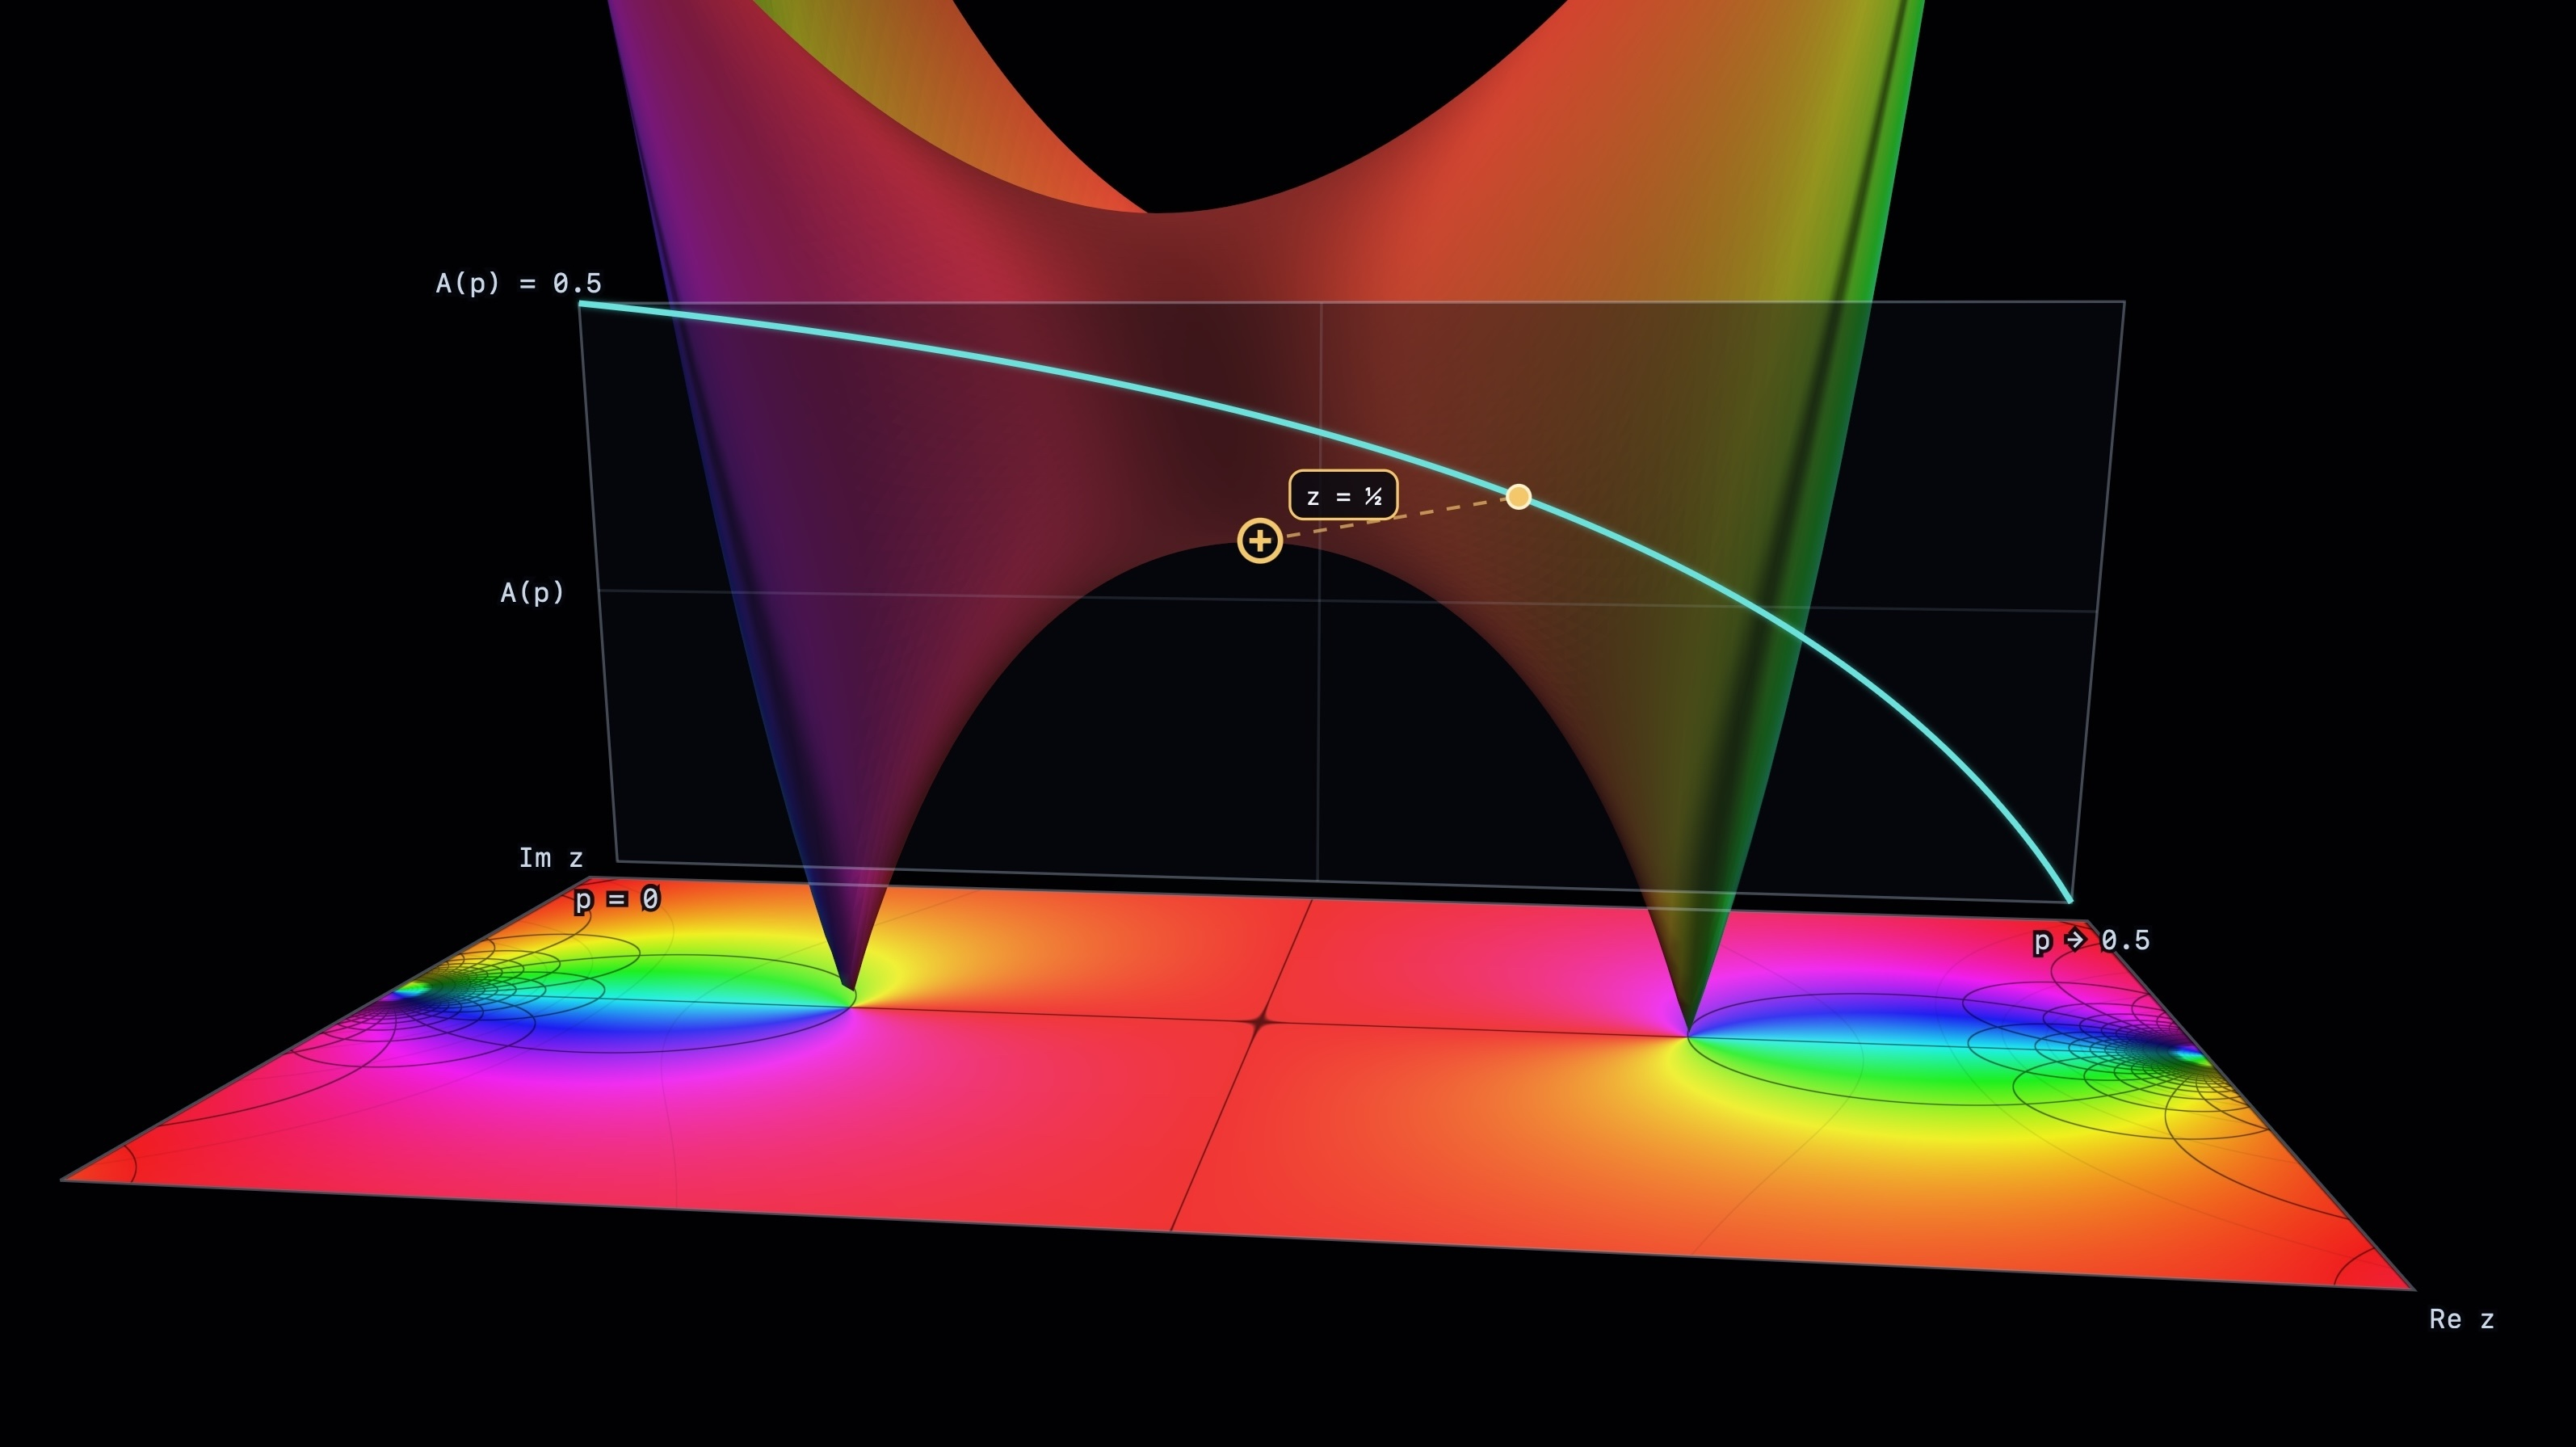
\includegraphics[width=\textwidth]{pictures/1B.jpg}
        \caption{The height at $z=\tfrac12$ against the $A(p)$ curve.}
    \end{subfigure}

    \caption[]{The Koenigs coordinate and $A(p)$ (continued on the following
    page).}
\end{figure}

The identity already established in Section~\ref{sec:koenigs},
\[
A(p)=2\psi_{2p}\!\left(\tfrac12\right),
\]
makes Figure~\ref{fig:koenigs-surface} the centre of this construction. For the
real branching slice $r=2p\in(0,1)$, the plotted height of $|2\psi_r(z)|$ above
$z=\tfrac12$ is $A(p)$; its reciprocal is the quasi-stationary mean from
Section~\ref{sec:limcondmean}, and its value is computed from the product of
Section~\ref{sec:product}. The cyan curve on the back panel traces the same
height as $p$ ranges over $(0,\tfrac12)$, while the dashed line joins its value
on that ordinary graph to the surface above the seed. The curve and the surface
are therefore two readings of the same value.

The branching initial condition fixes the seed: $S_0=1$ gives
$w_0=\tfrac12$. This is also the critical point of the logistic map because
\[
f_r'(z)=r(1-2z)
\]
vanishes there. The two funnels descend to the zeros $\psi_r(0)=\psi_r(1)=0$,
at the attracting fixed point and its other preimage $f_r(1)=0$; the same two
zeros flank the marker on the later coordinate plates. Thus the scalar $A(p)$
is one distinguished value of the analytic coordinate drawn across the whole
basin.

\begin{figure}[!t]
    \ContinuedFloat
    \centering

    \begin{subfigure}[b]{0.57\textwidth}
        \centering
        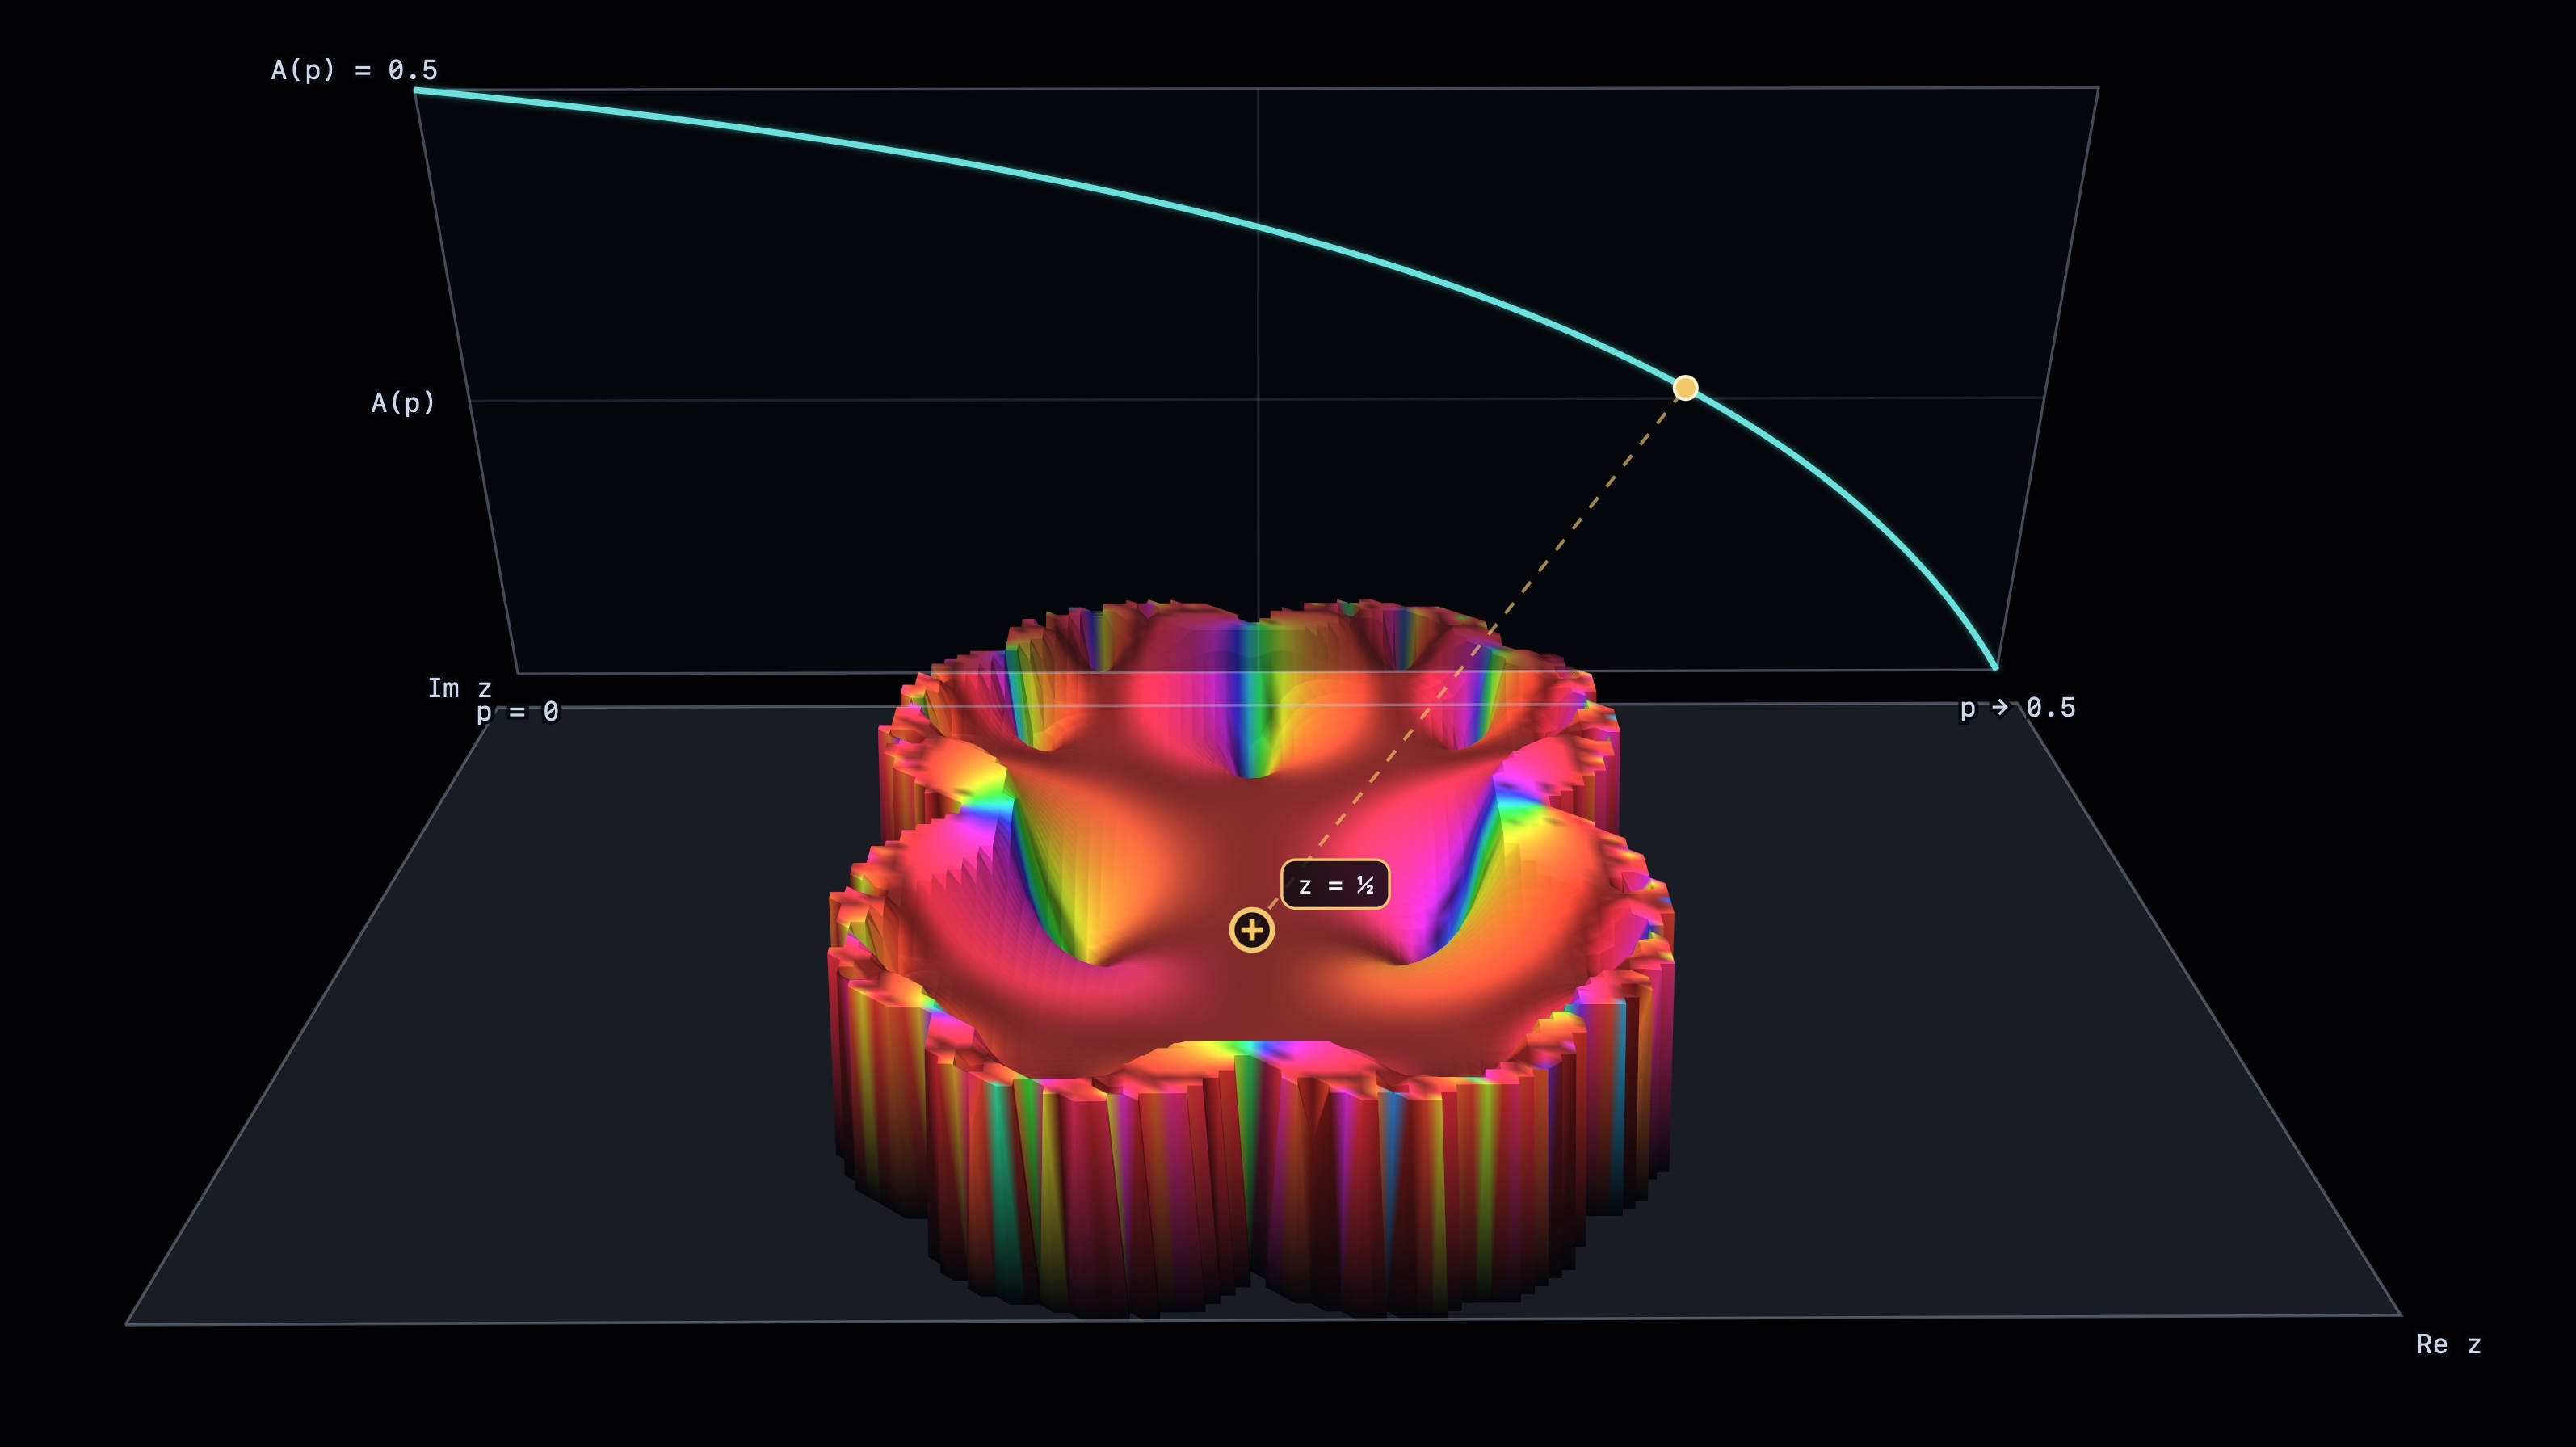
\includegraphics[width=\textwidth]{pictures/2B.jpg}
        \caption{The same surface viewed from lower down.}
    \end{subfigure}

    \vspace{3pt}
    \begin{subfigure}[b]{0.57\textwidth}
        \centering
        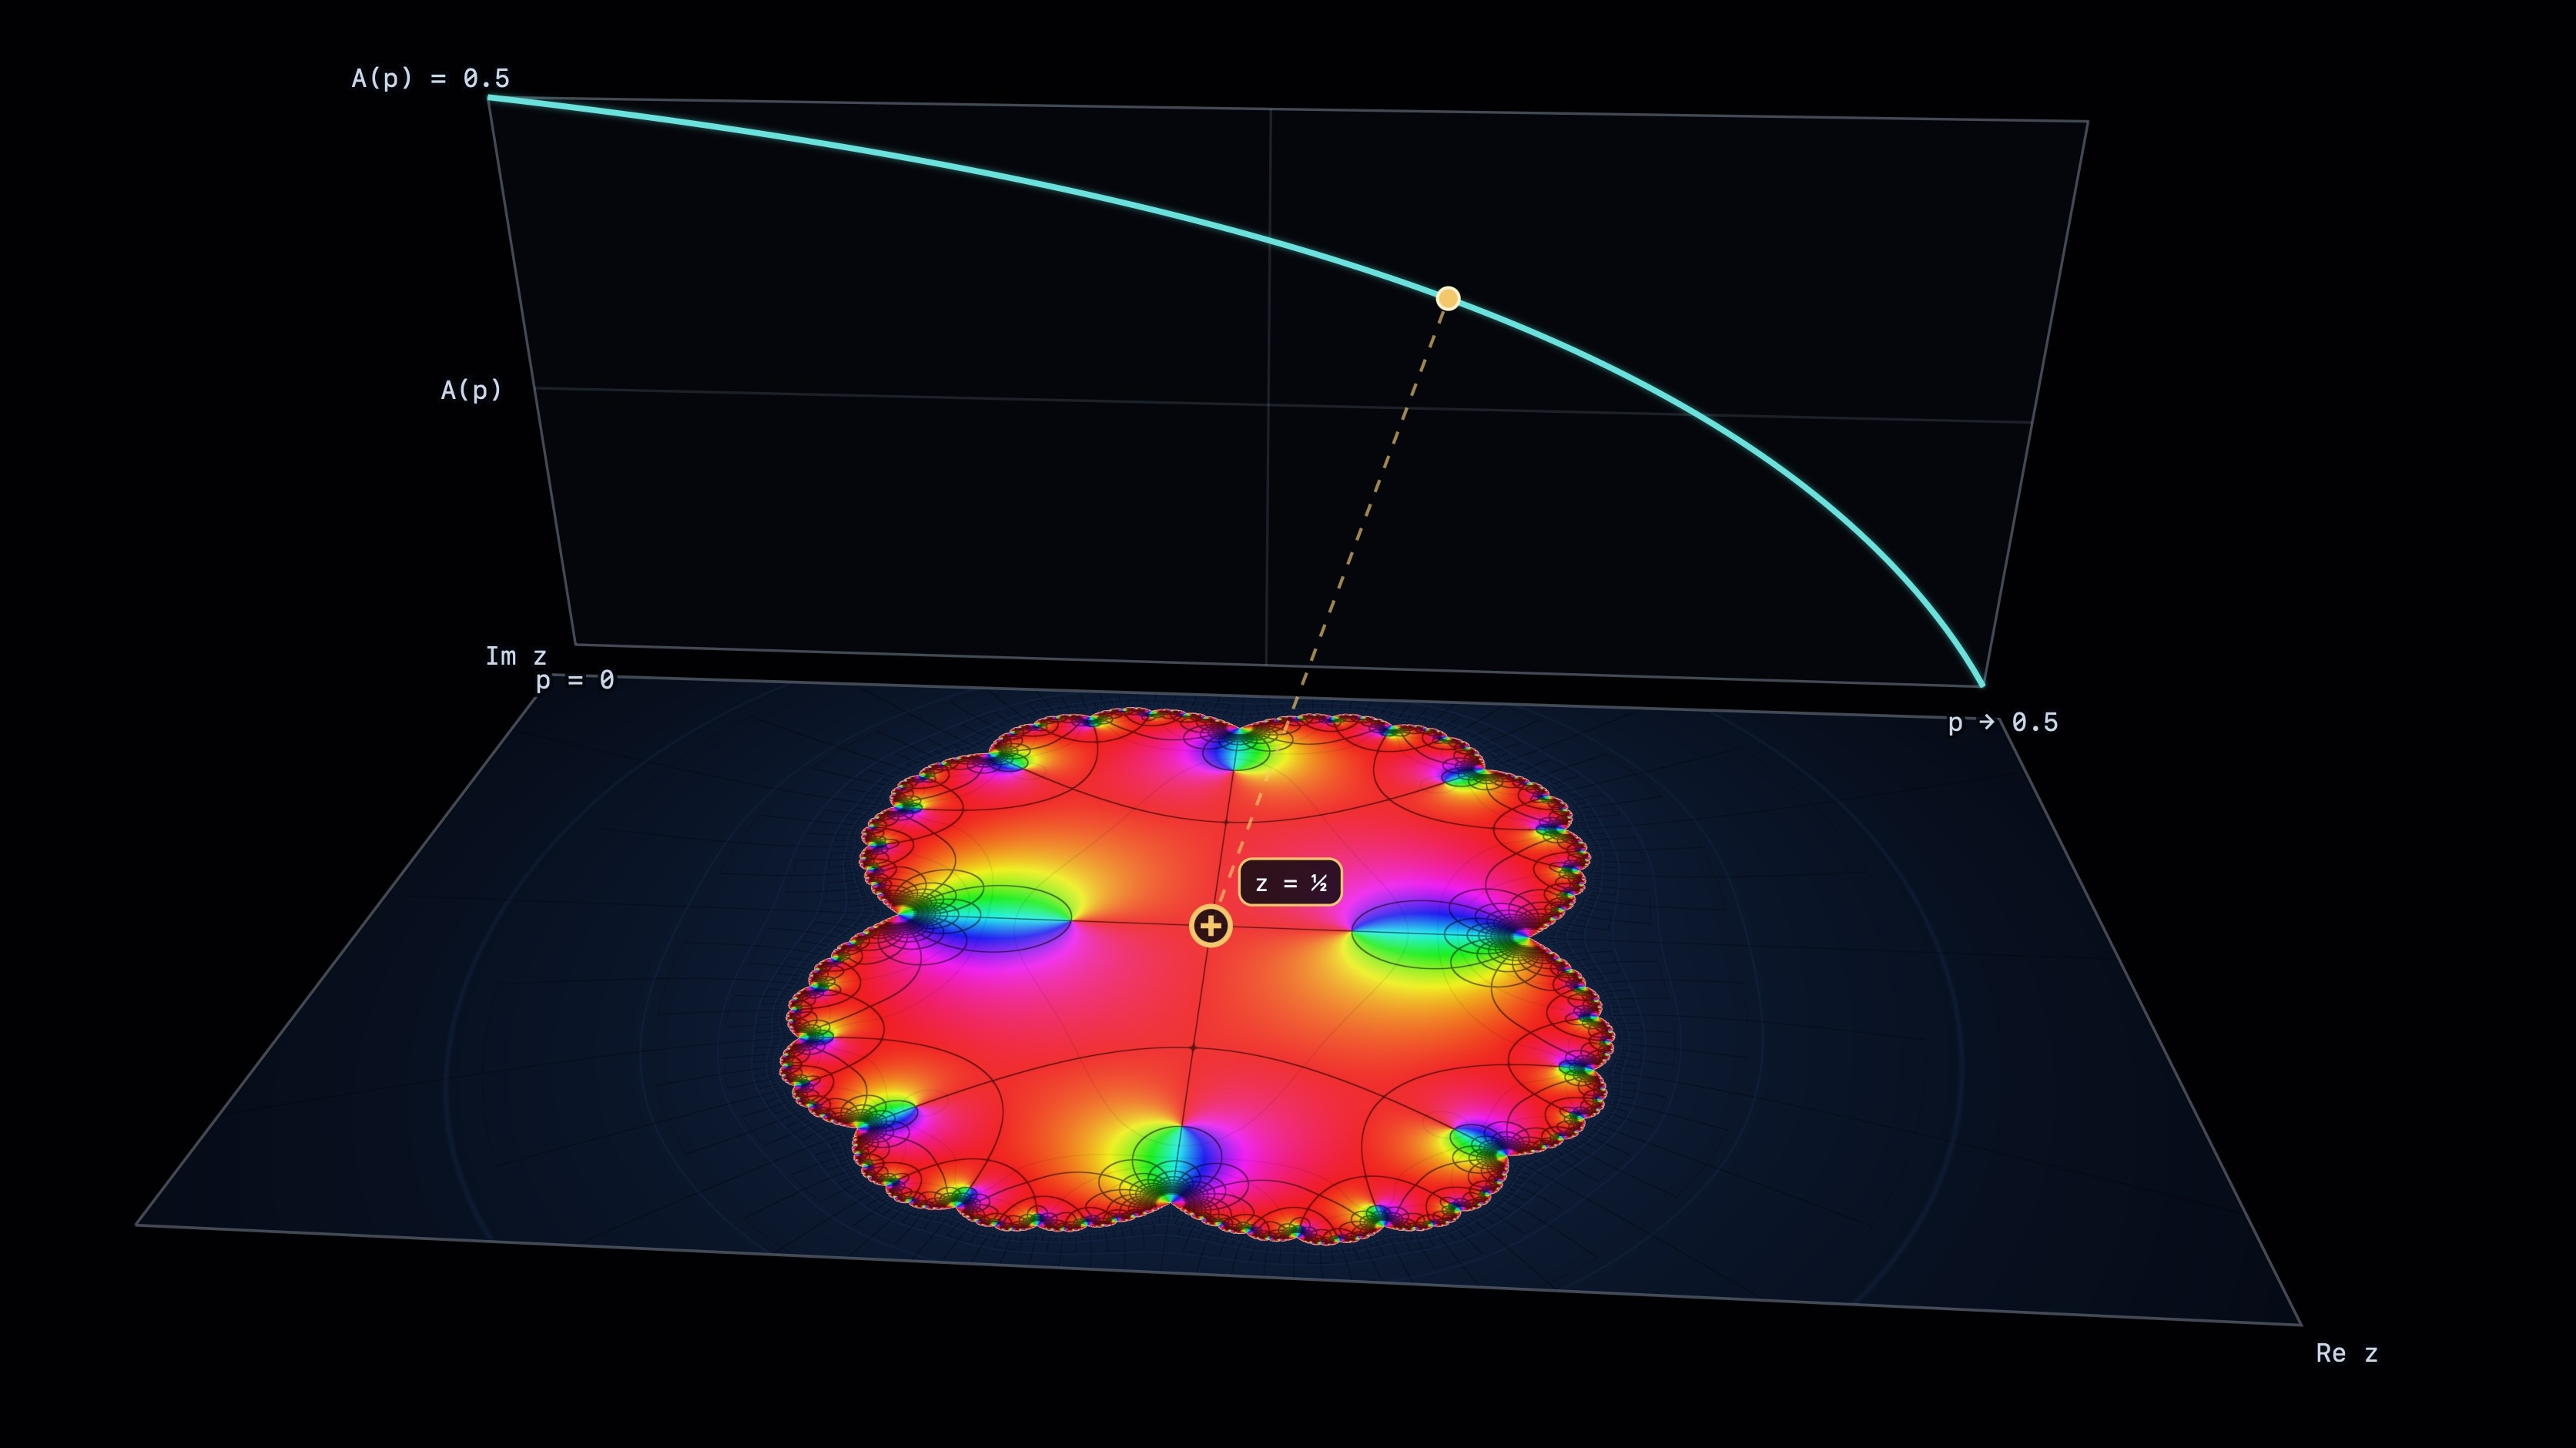
\includegraphics[width=\textwidth]{pictures/3B.jpg}
        \caption{The raised surface removed.}
    \end{subfigure}

    \caption{The Koenigs coordinate at $r=0.64$ ($p=0.32$). In (a), the marked
    seed $z=\tfrac12$ has product-computed height $A(p)=0.335521$ on
    $|2\psi_r(z)|$; the dashed line matches it to the cyan $A$-against-$p$
    curve. Panels (b) and (c) lower and remove the surface. The funnels mark
    $\psi_r(0)=\psi_r(1)=0$, and the reciprocal height gives the
    quasi-stationary mean $1/A(p)=2.980439$.}
    \label{fig:koenigs-surface}
\end{figure}

\FloatBarrier

\subsection{Leaving the real branching slice}

The branching problem occupies a one-real-dimensional slice of the
two-real-dimensional $r$-plane. Figure~\ref{fig:koenigs-seq} begins with
$r=2p=0.64$, the branching case $p=0.32$, and then gives $r$ a growing
imaginary part. More generally, Koenigs' construction supplies $\psi_r$ for
every multiplier with $0<|r|<1$, whereas the probabilistic reading requires
$r$ to lie on the open real segment $(0,1)$. In panels (b)--(e), $|r|<1$: the
origin remains attracting, the Koenigs coordinate and its basin remain well
defined, and the figures retain their complex-dynamical meaning. What is lost
is the probability model. Once $r/2$ is not real in $(0,\tfrac12)$, it is not a
branching probability, so these panels are analytic continuation in the
parameter rather than new probabilistic cases. The change is in interpretation,
not in the analytic construction.

Panel (f) crosses the boundary of this construction. There
$r=0.64-0.78i$ has $|r|\approx1.009>1$, the origin is no longer attracting, and
the attracting Koenigs chart used above no longer applies.

\begin{figure}[htbp]
    \centering
    \begin{subfigure}[b]{0.32\textwidth}
        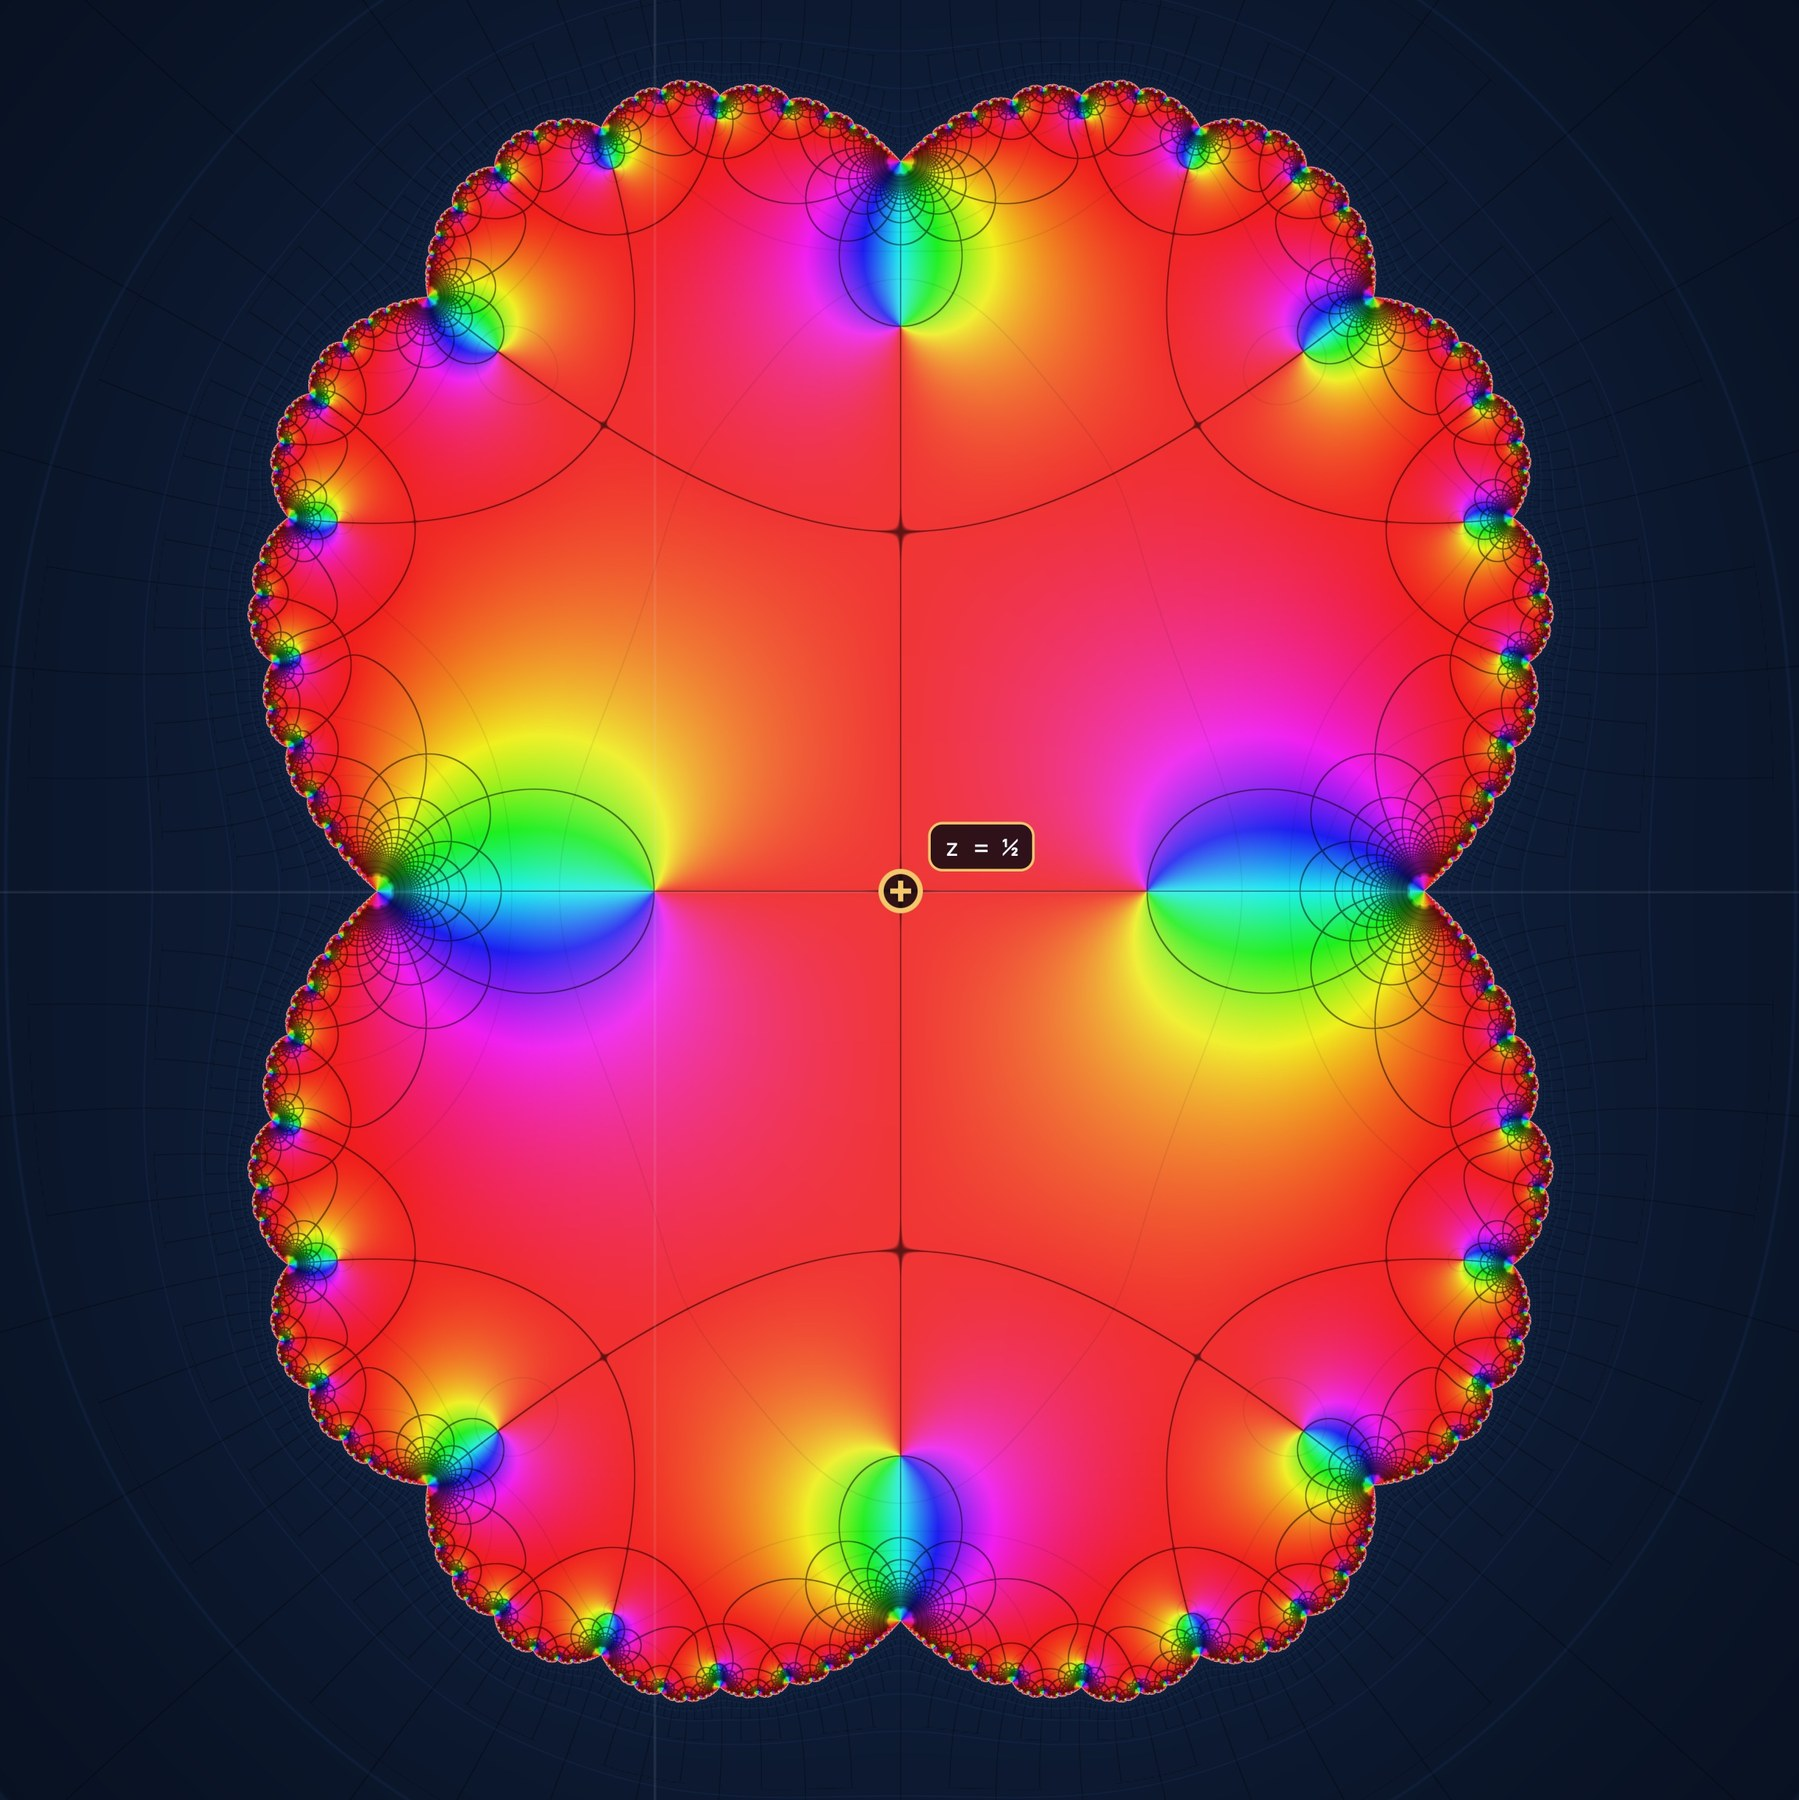
\includegraphics[width=\textwidth]{pictures/koenigs_seq_4a.jpg}
        \caption{$r=0.64$}
    \end{subfigure}
    \hfill
    \begin{subfigure}[b]{0.32\textwidth}
        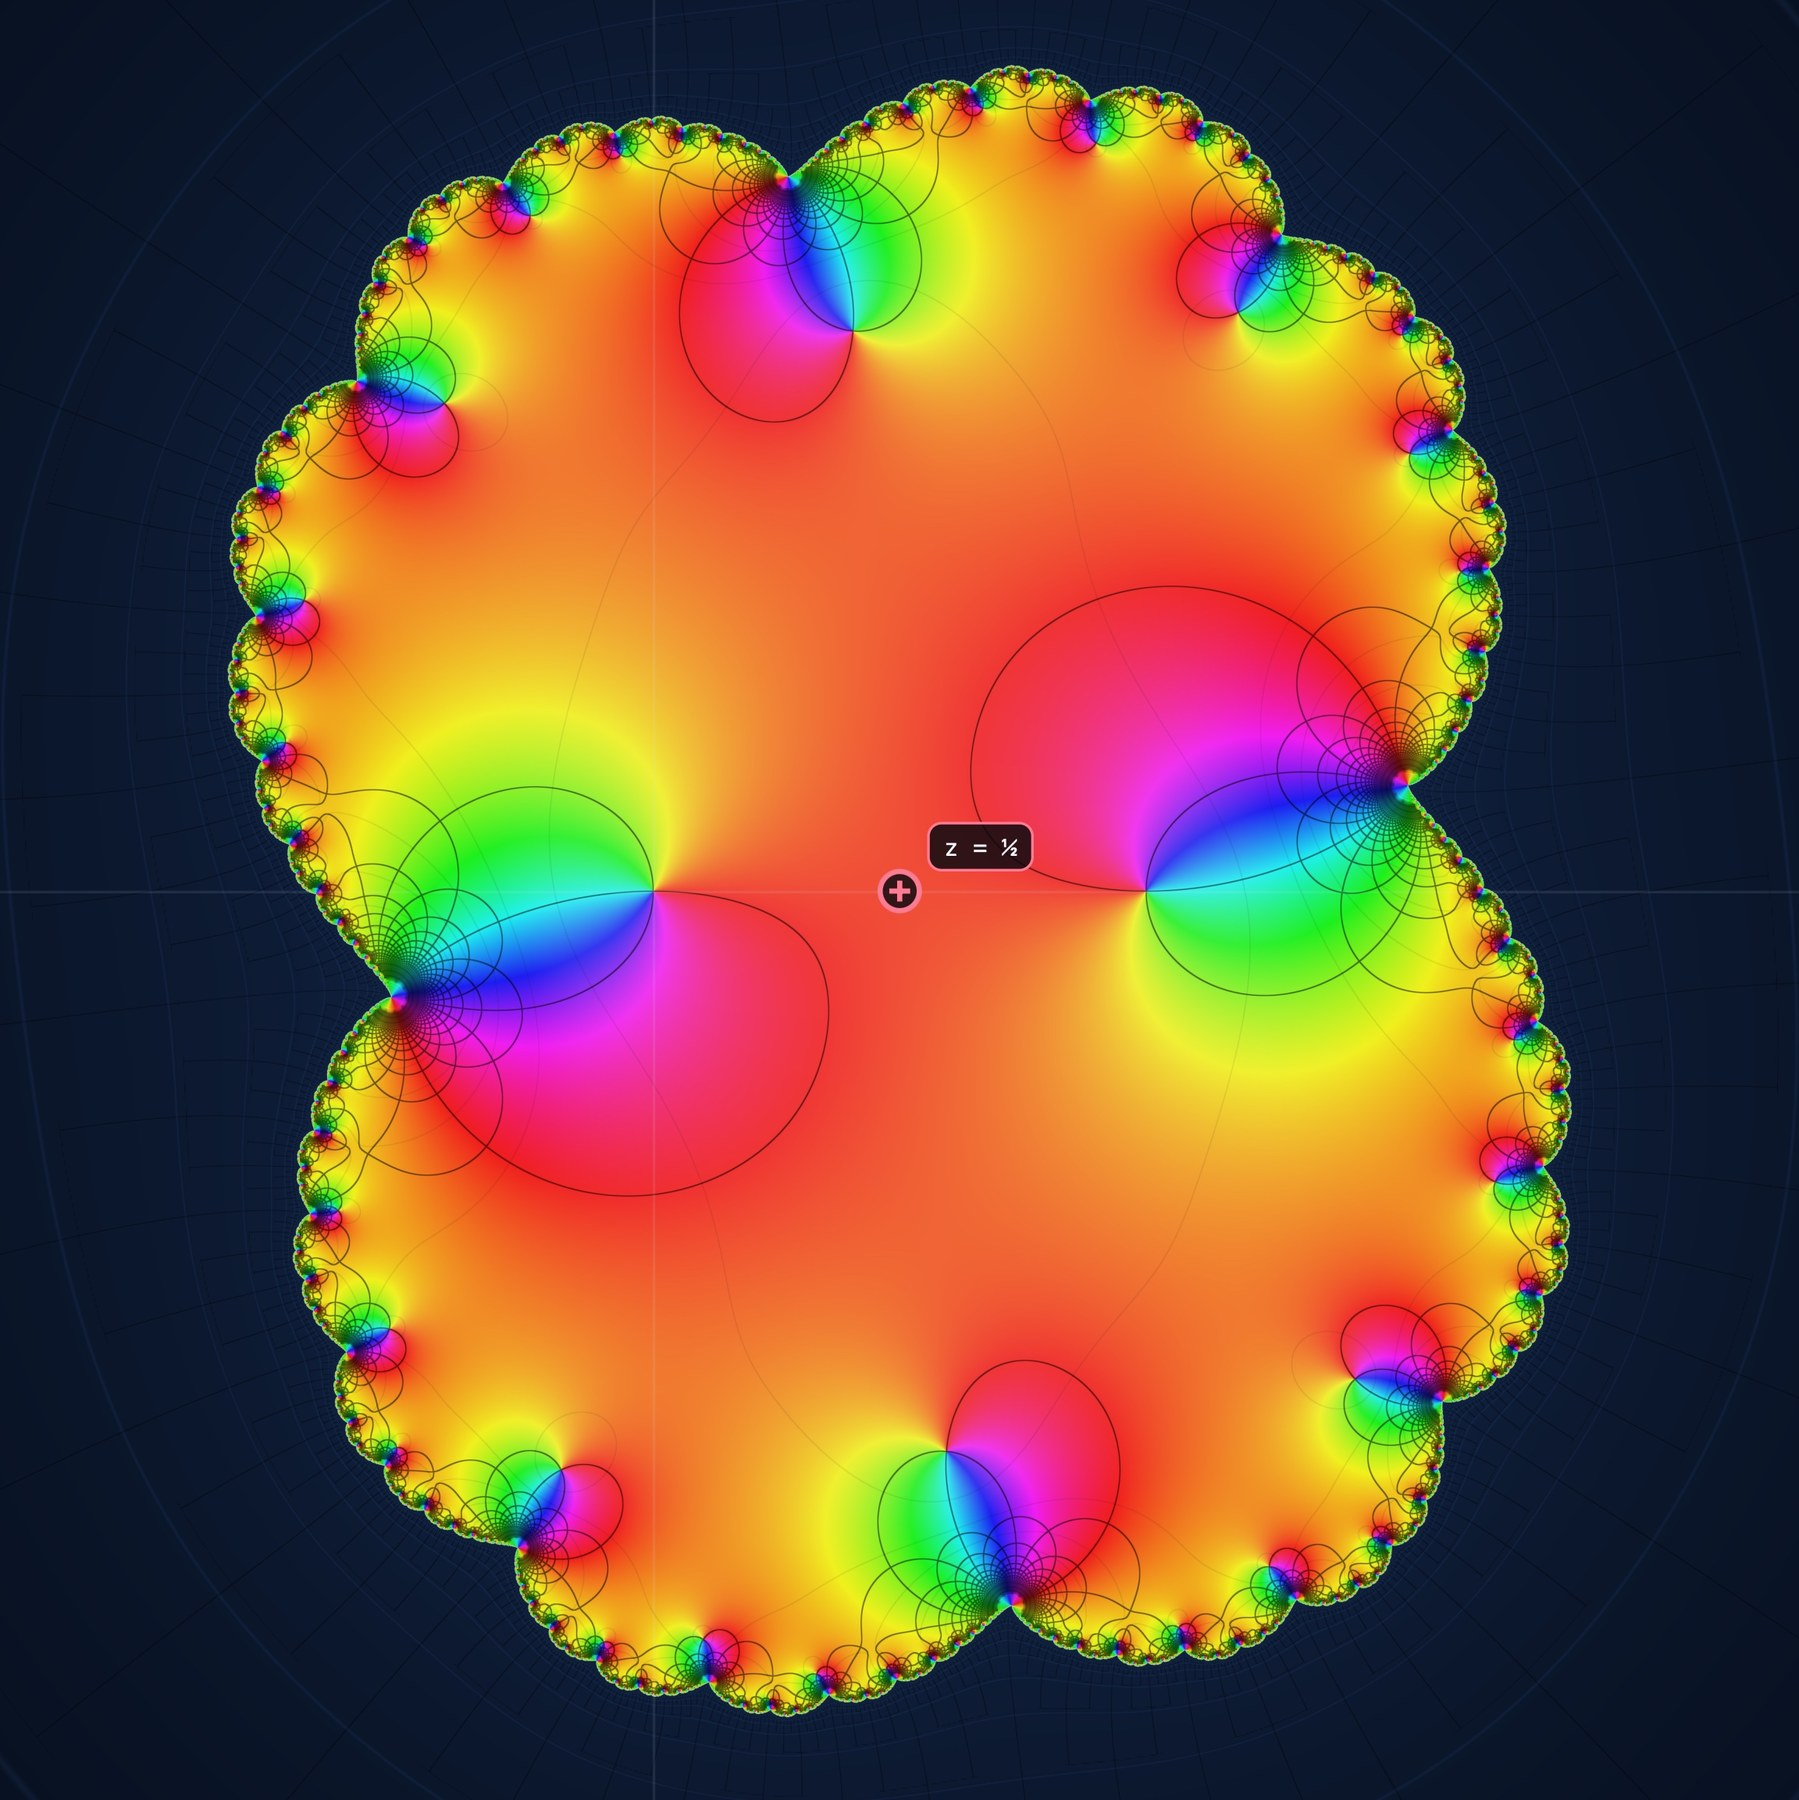
\includegraphics[width=\textwidth]{pictures/koenigs_seq_4b.jpg}
        \caption{$r=0.64-0.09i$}
    \end{subfigure}
    \hfill
    \begin{subfigure}[b]{0.32\textwidth}
        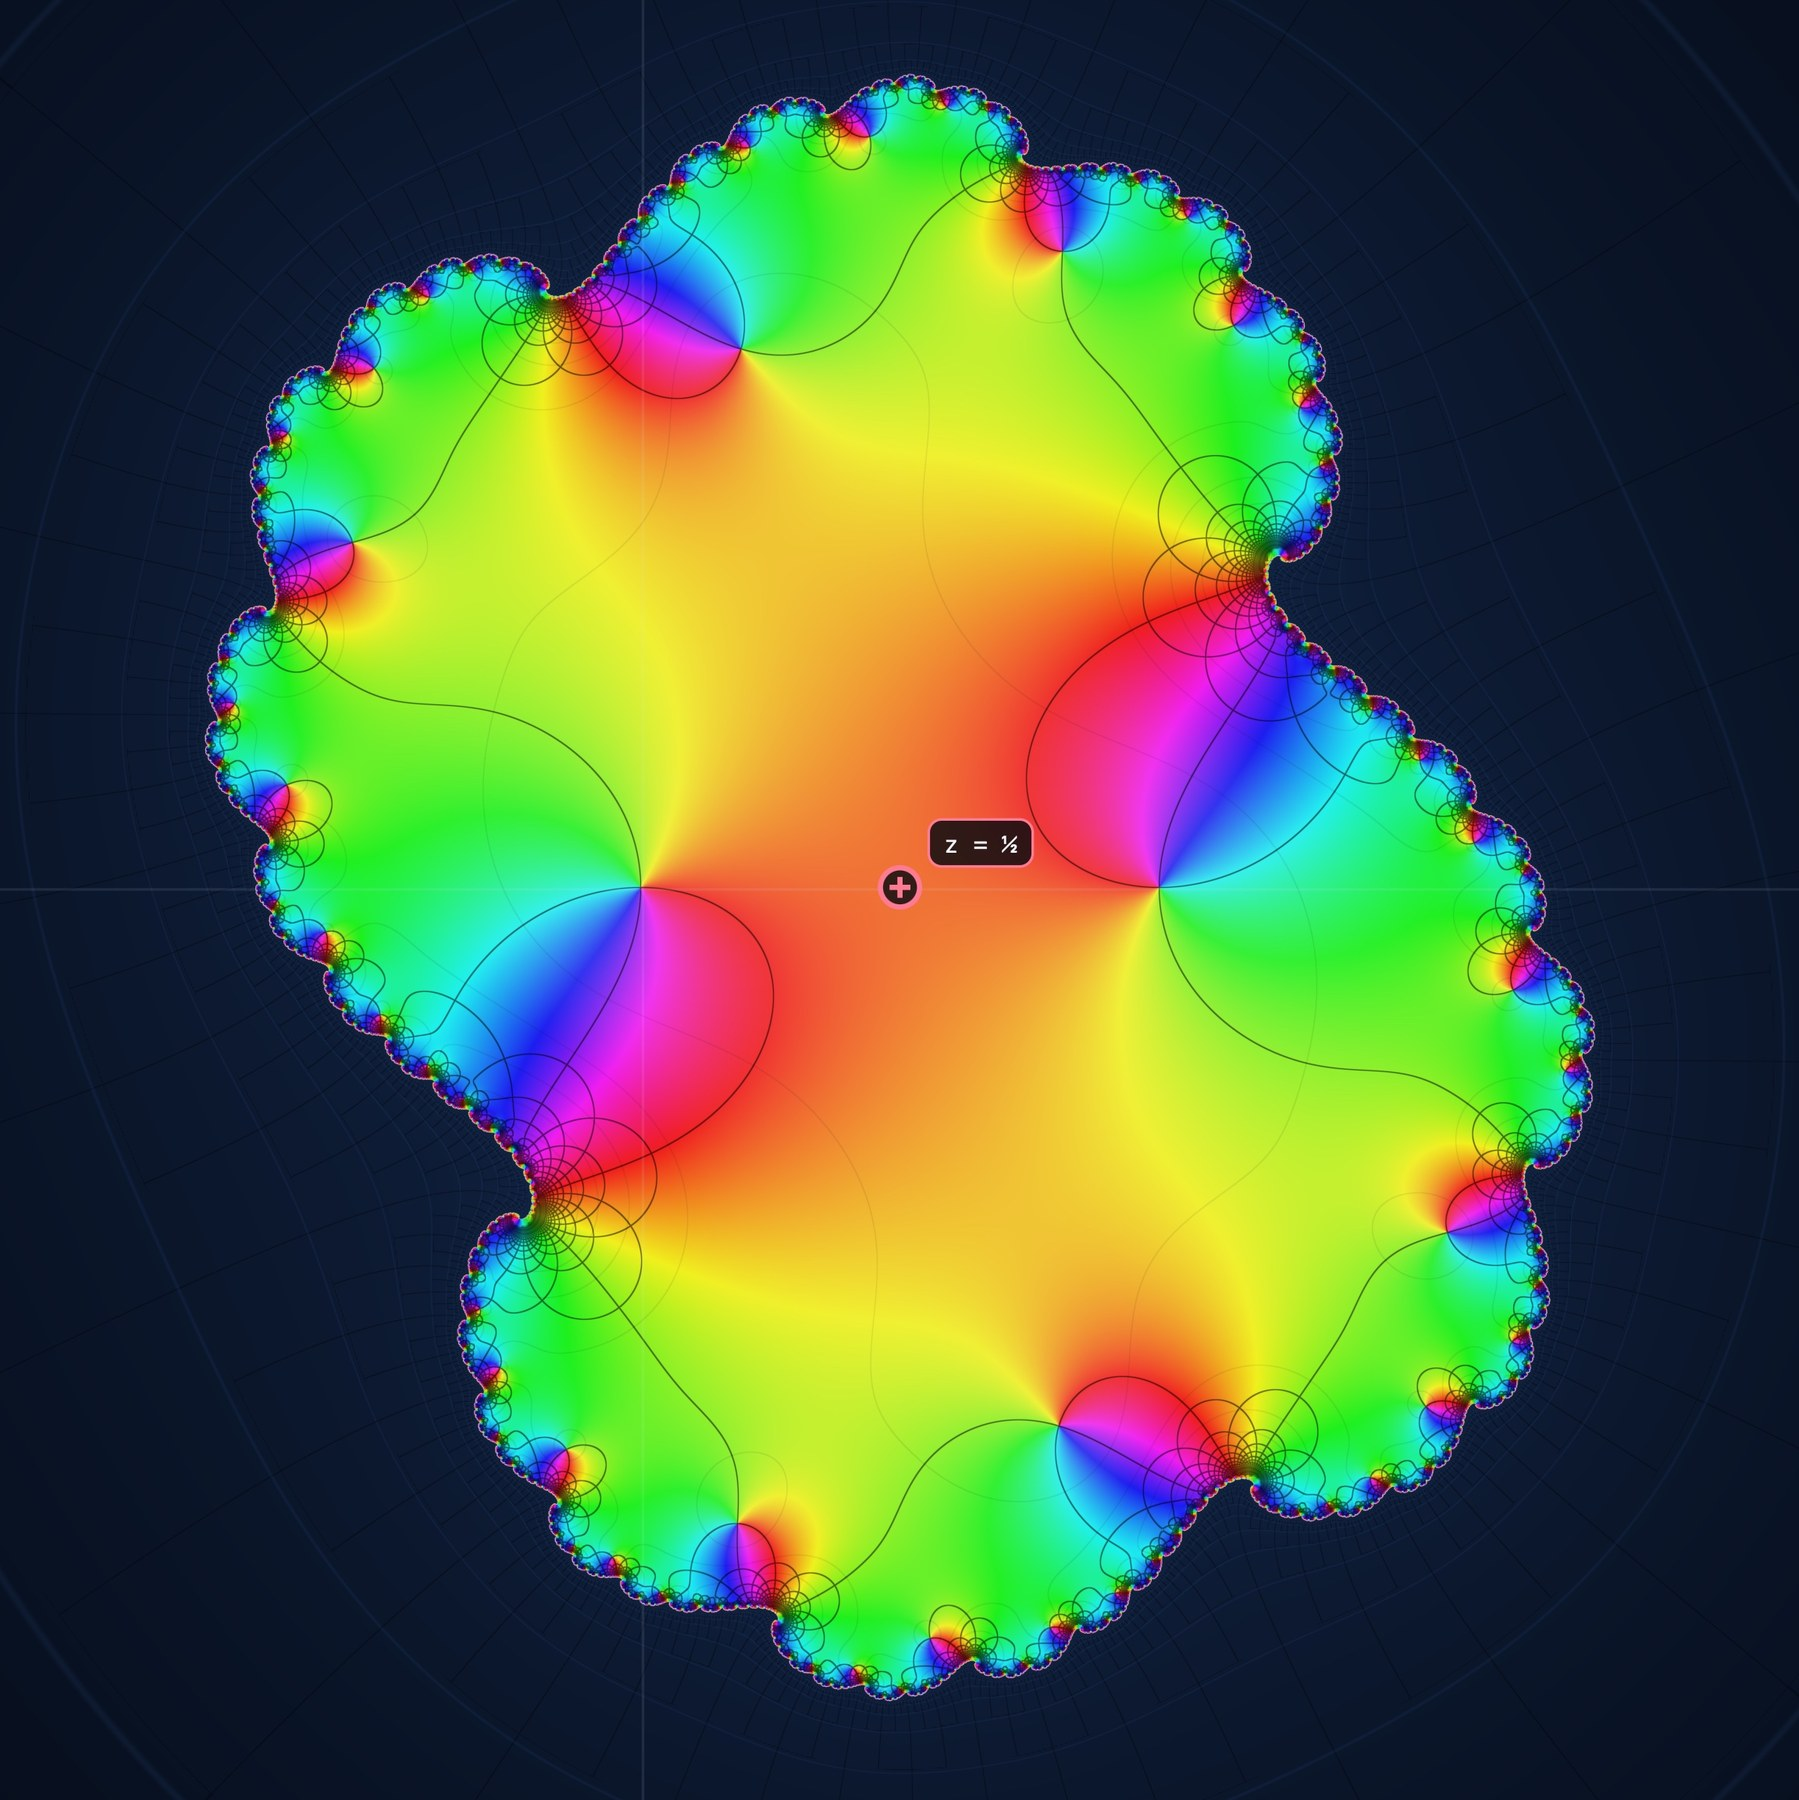
\includegraphics[width=\textwidth]{pictures/koenigs_seq_4c.jpg}
        \caption{$r=0.64-0.33i$}
    \end{subfigure}

    \vspace{6pt}
    \begin{subfigure}[b]{0.32\textwidth}
        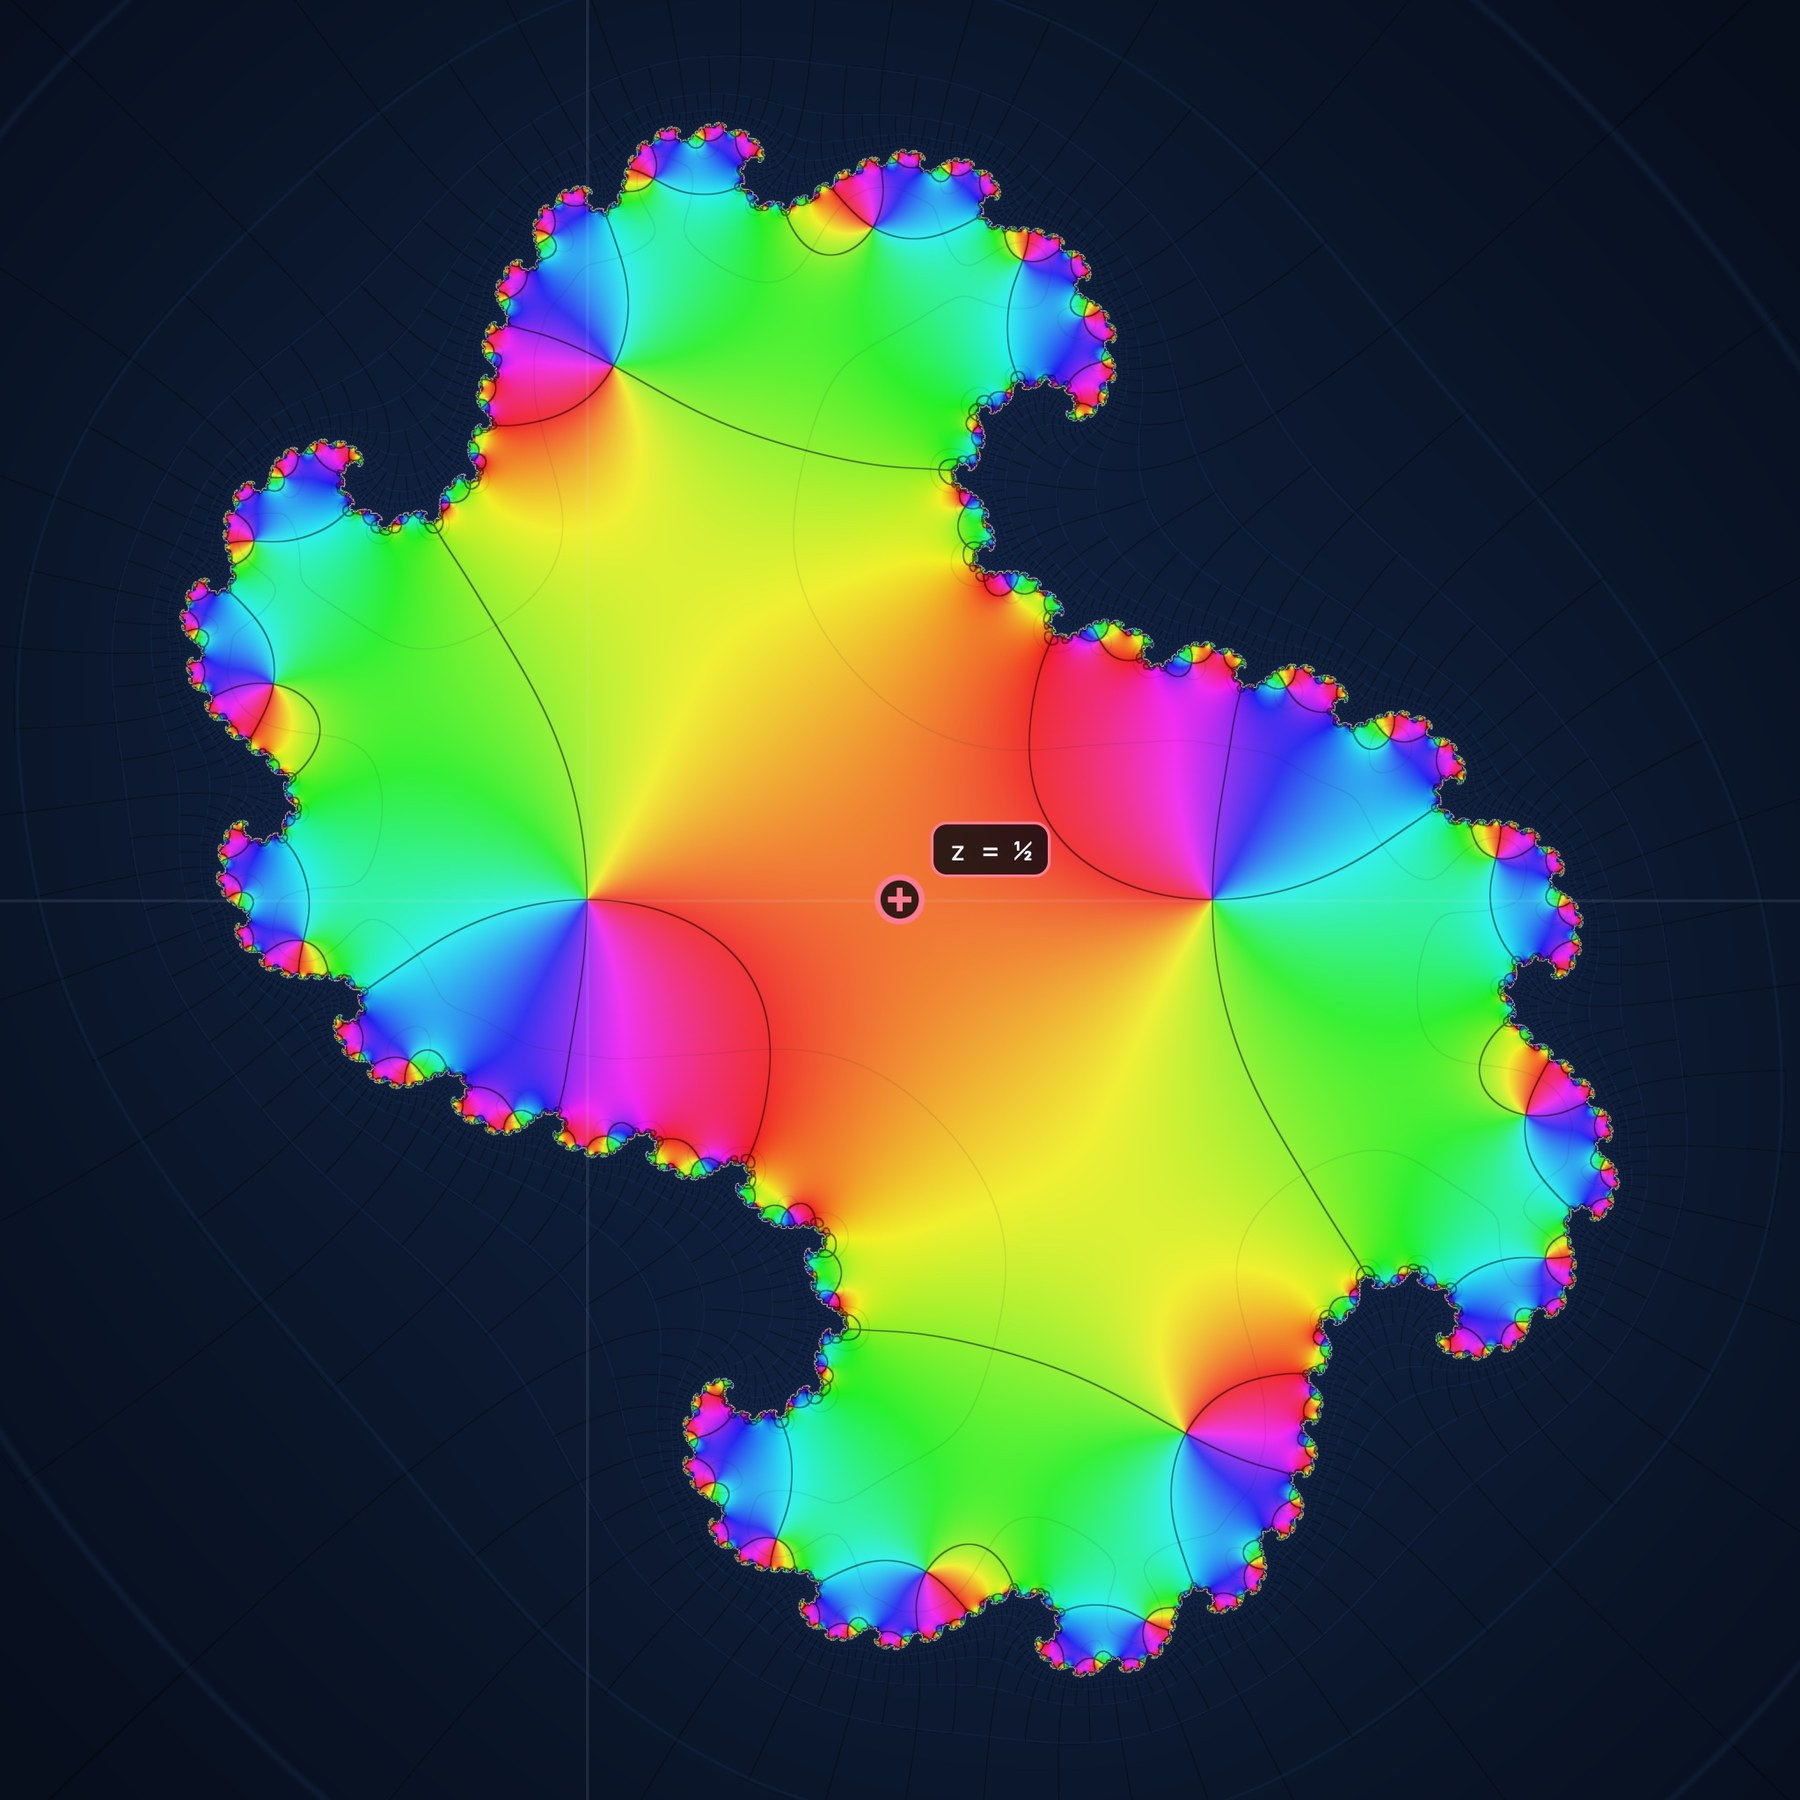
\includegraphics[width=\textwidth]{pictures/koenigs_seq_4d.jpg}
        \caption{$r=0.64-0.65i$}
    \end{subfigure}
    \hfill
    \begin{subfigure}[b]{0.32\textwidth}
        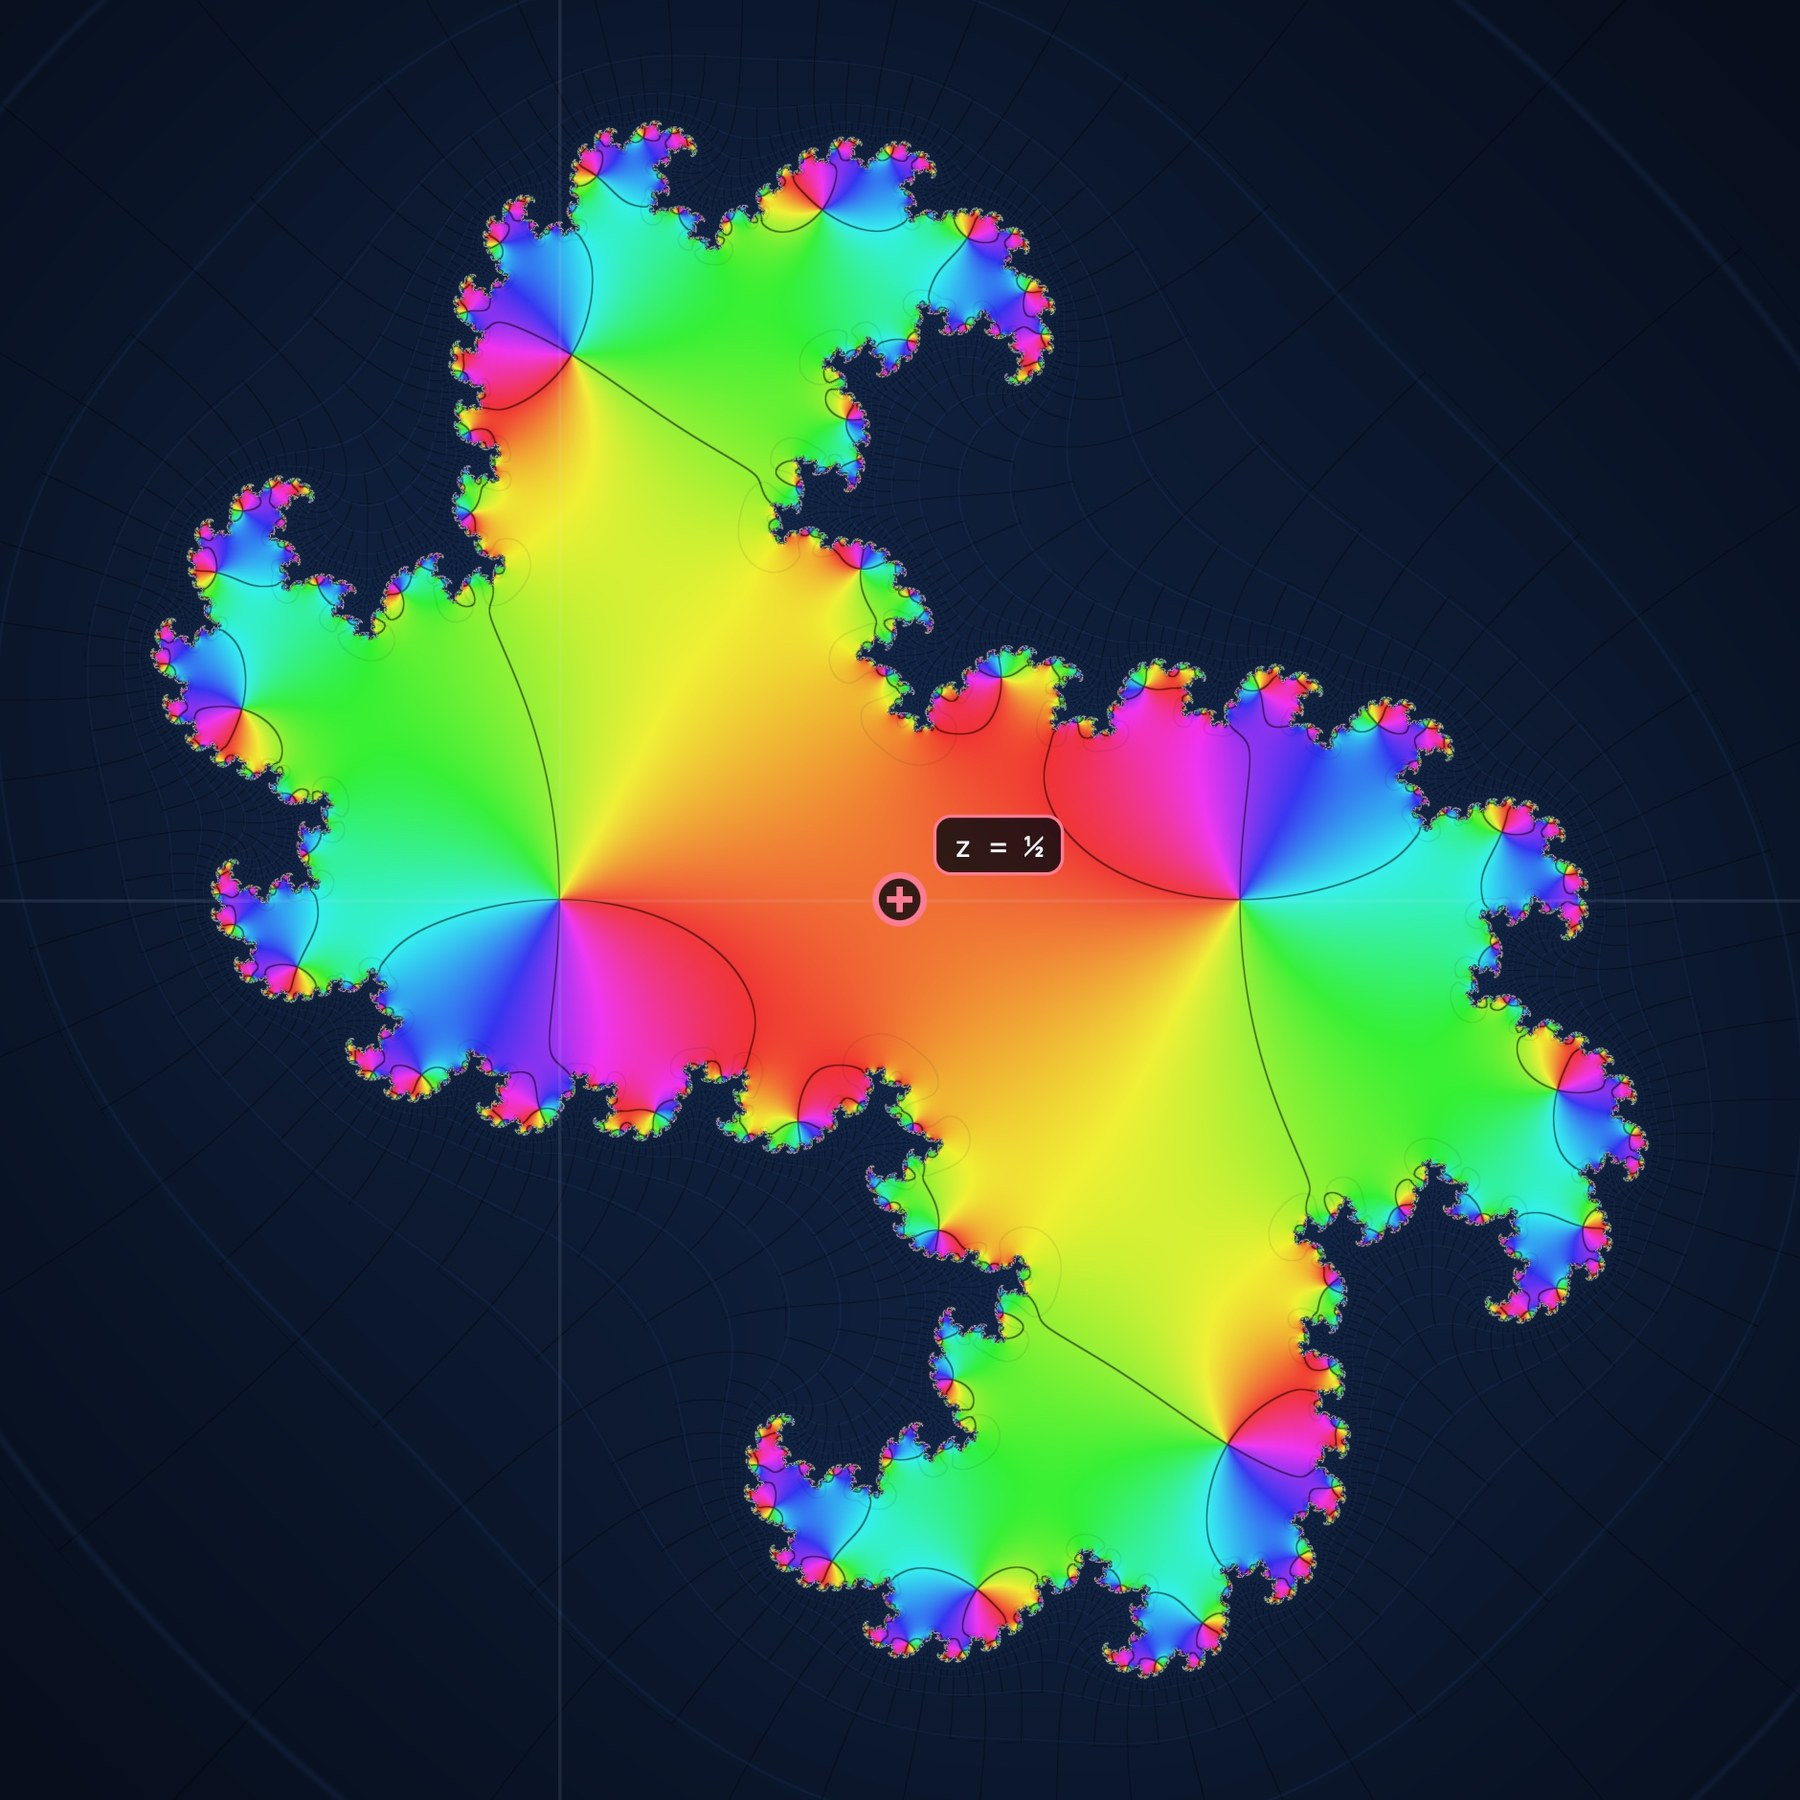
\includegraphics[width=\textwidth]{pictures/koenigs_seq_4e.jpg}
        \caption{$r=0.64-0.75i$}
    \end{subfigure}
    \hfill
    \begin{subfigure}[b]{0.32\textwidth}
        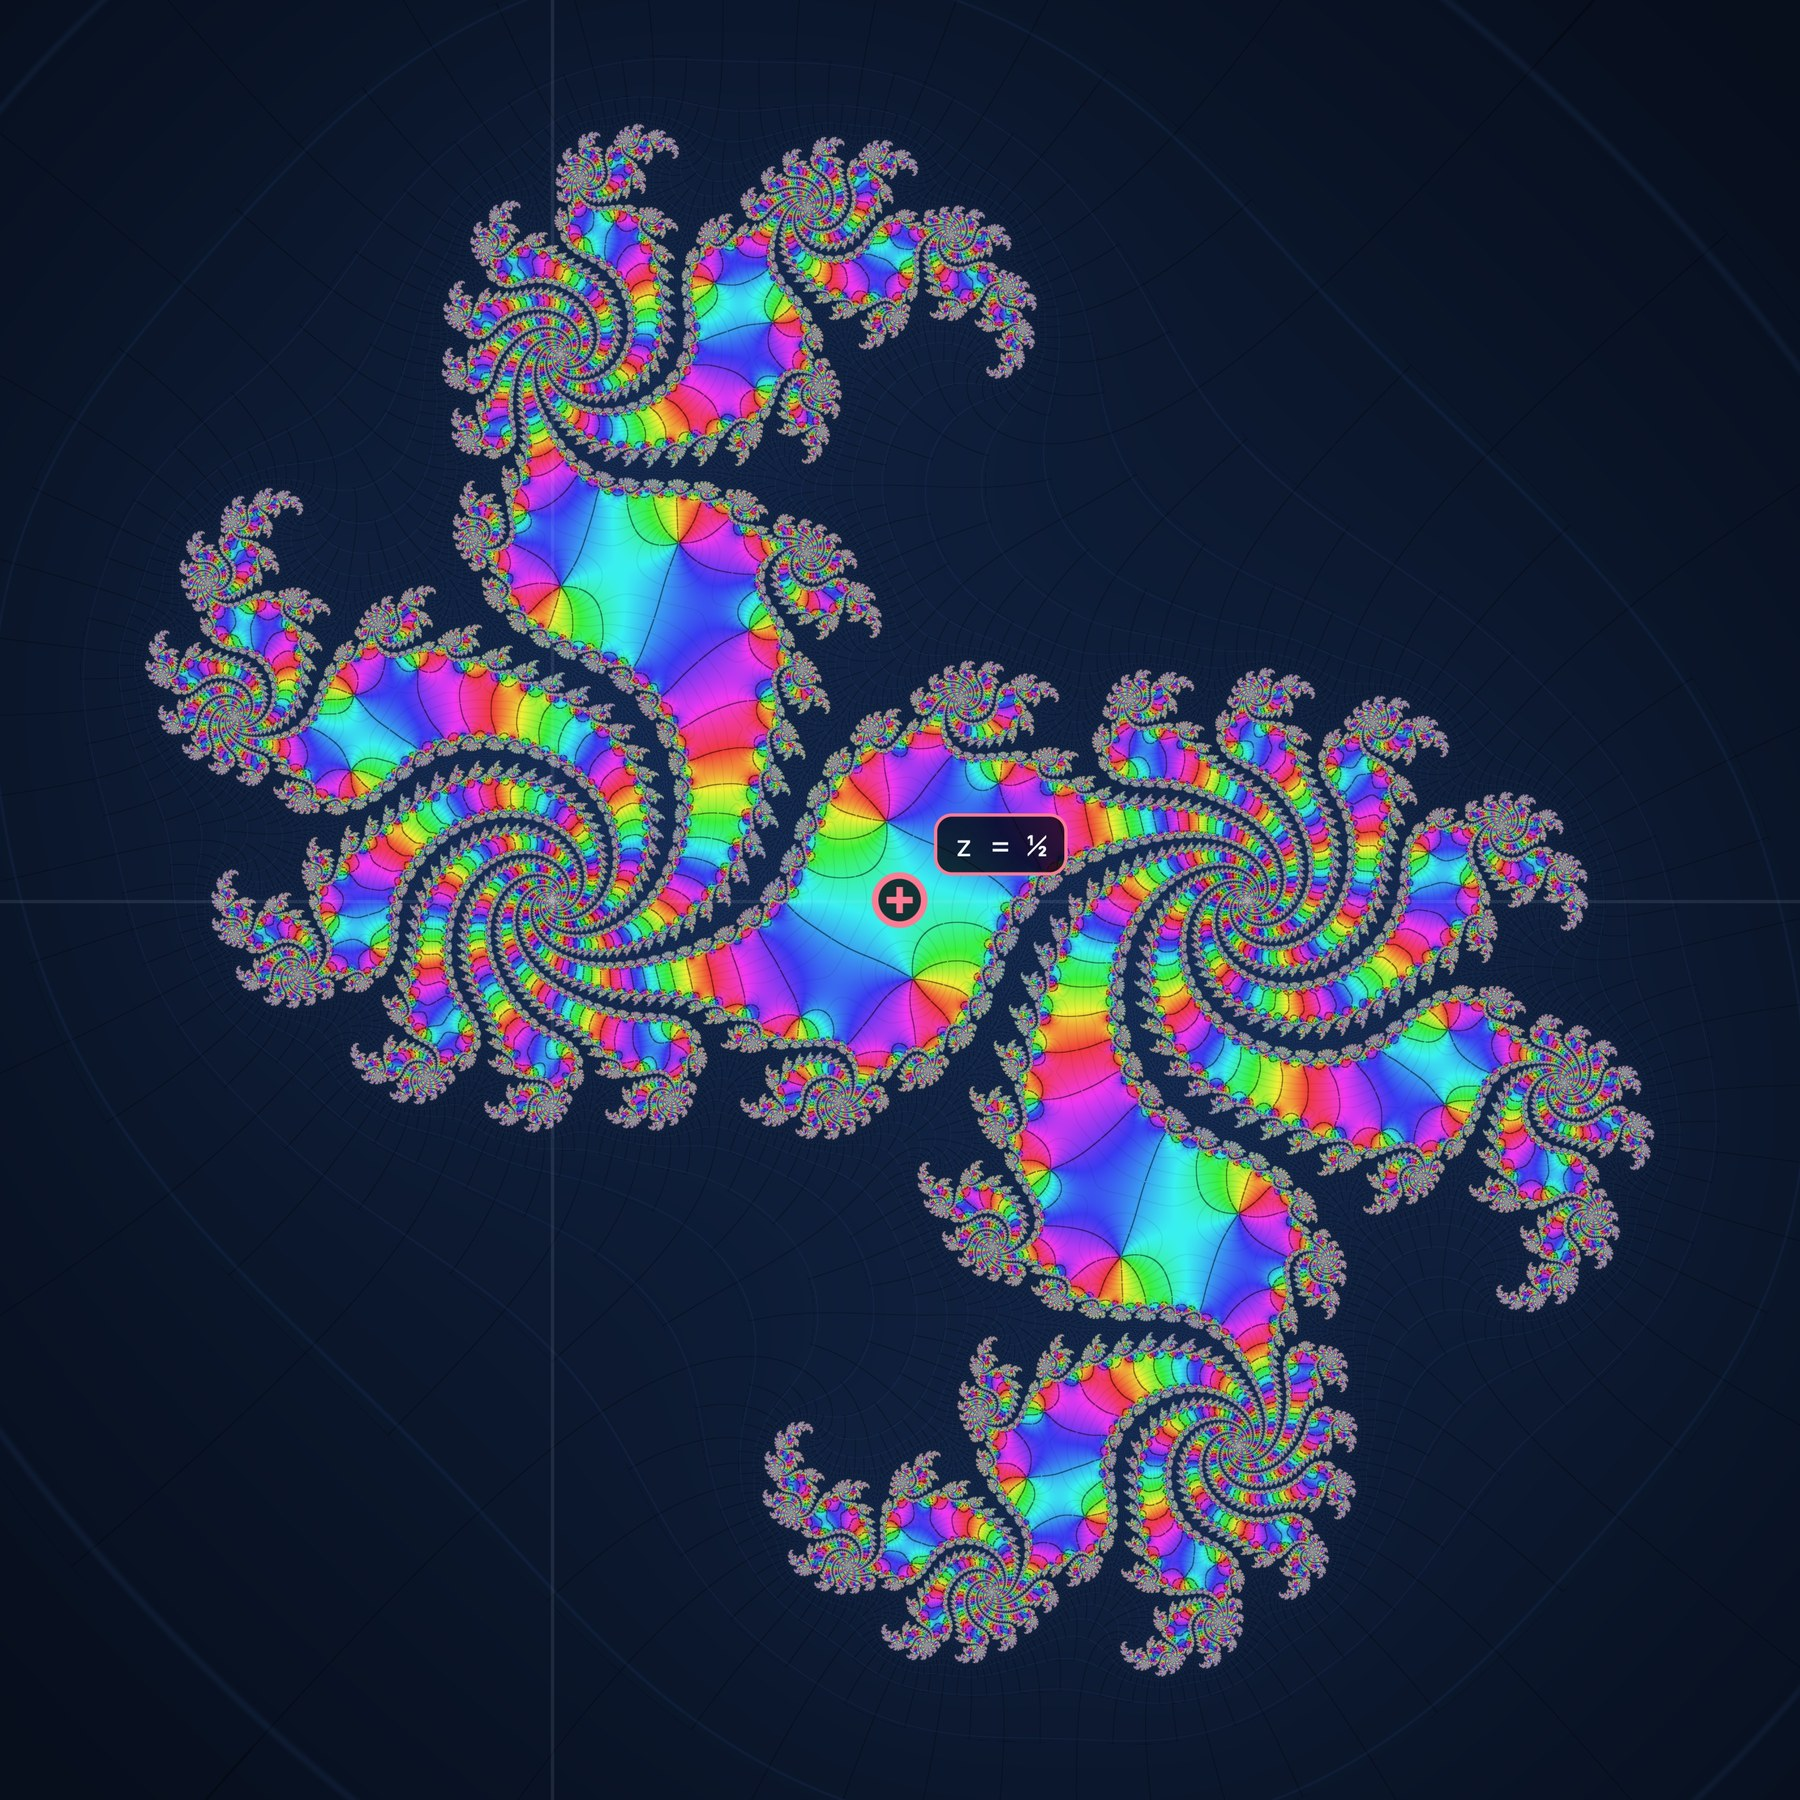
\includegraphics[width=\textwidth]{pictures/koenigs_seq_4f.jpg}
        \caption{$r=0.64-0.78i$}
    \end{subfigure}

    \caption{Continuation from the real branching slice at
    $\operatorname{Re}r=0.64$. Panel (a) is the branching case $p=0.32$, with
    $A(p)=0.335521$ and $1/A(p)=2.980439$. In (b)--(e), $|r|$ is $0.646$,
    $0.720$, $0.912$ and $0.986$: the Koenigs coordinate persists, but $r/2$ is
    no longer a probability. In (f), $|r|\approx1.009$ and the attracting chart
    no longer applies. The marked point is $z=\tfrac12$ throughout.}
    \label{fig:koenigs-seq}
\end{figure}

\FloatBarrier

\begin{figure}[p]
    \centering
    \begin{subfigure}[b]{0.48\textwidth}
        
\includegraphics[width=\textwidth]{pictures/koenigs_gallery_3.jpg}
        \caption{$r=-0.00048+1.14725i$}
    \end{subfigure}
    \hfill
    \begin{subfigure}[b]{0.48\textwidth}
        
\includegraphics[width=\textwidth]{pictures/koenigs_gallery_1.jpg}
        \caption{$r=-1.582$}
    \end{subfigure}

    \vspace{5pt}
    \begin{subfigure}[b]{0.48\textwidth}
        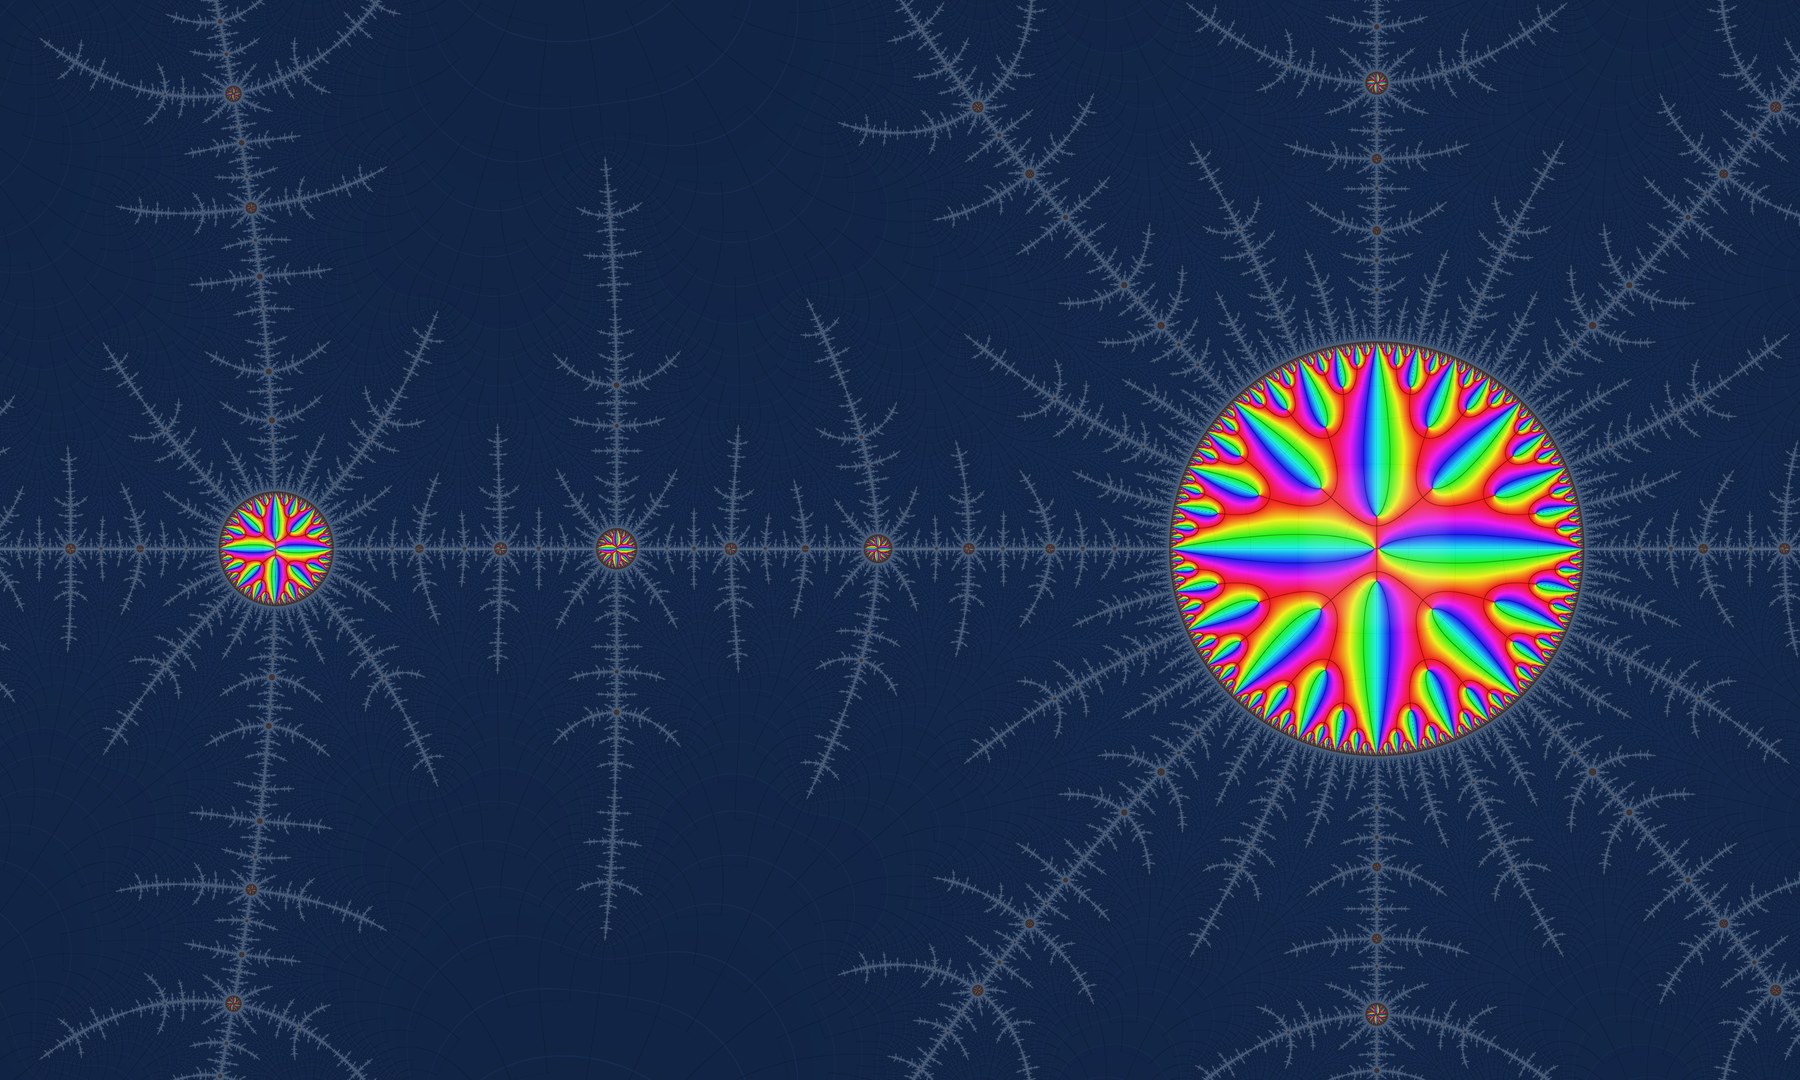
\includegraphics[width=\textwidth]{pictures/koenigs_gallery_Ka.jpg}
        \caption{$r=-1.5822$}
    \end{subfigure}
    \hfill
    \begin{subfigure}[b]{0.48\textwidth}
        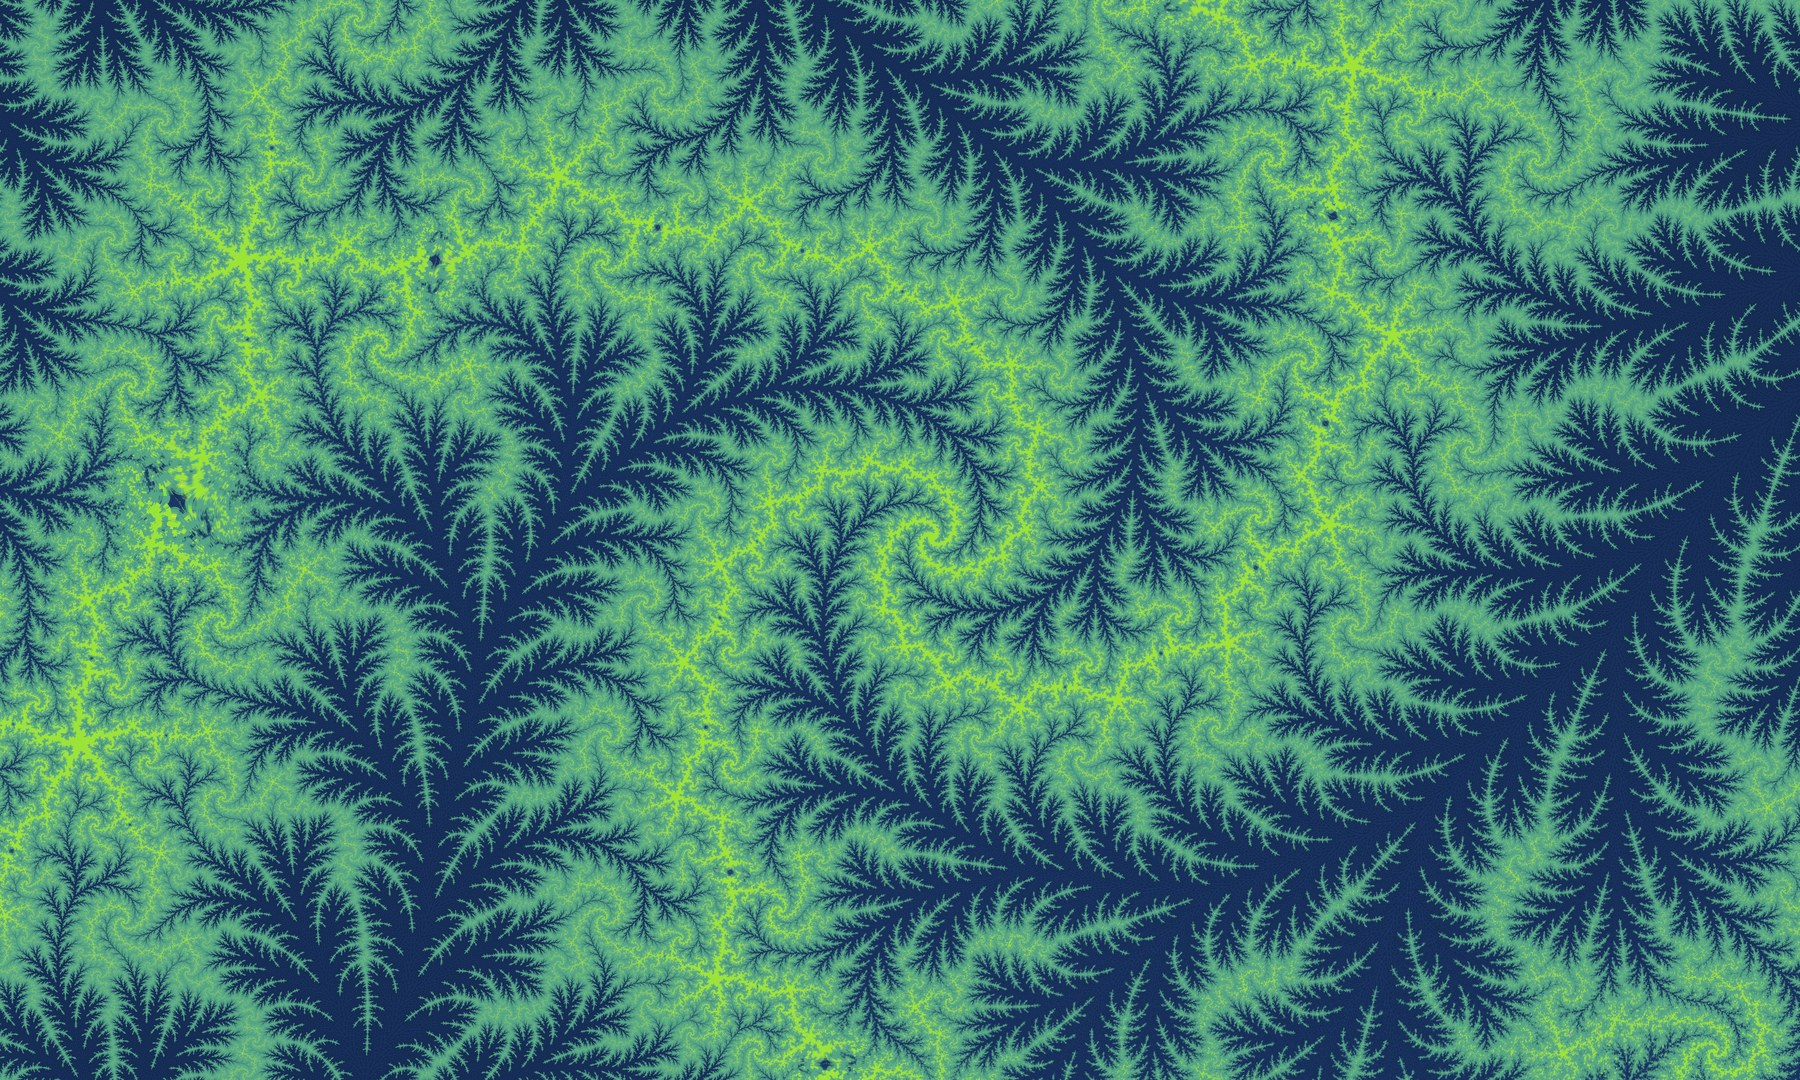
\includegraphics[width=\textwidth]{pictures/koenigs_gallery_Kb.jpg}
        \caption{$r=-1.568+0.00179i$}
    \end{subfigure}

    \vspace{5pt}
    \begin{subfigure}[b]{0.48\textwidth}
        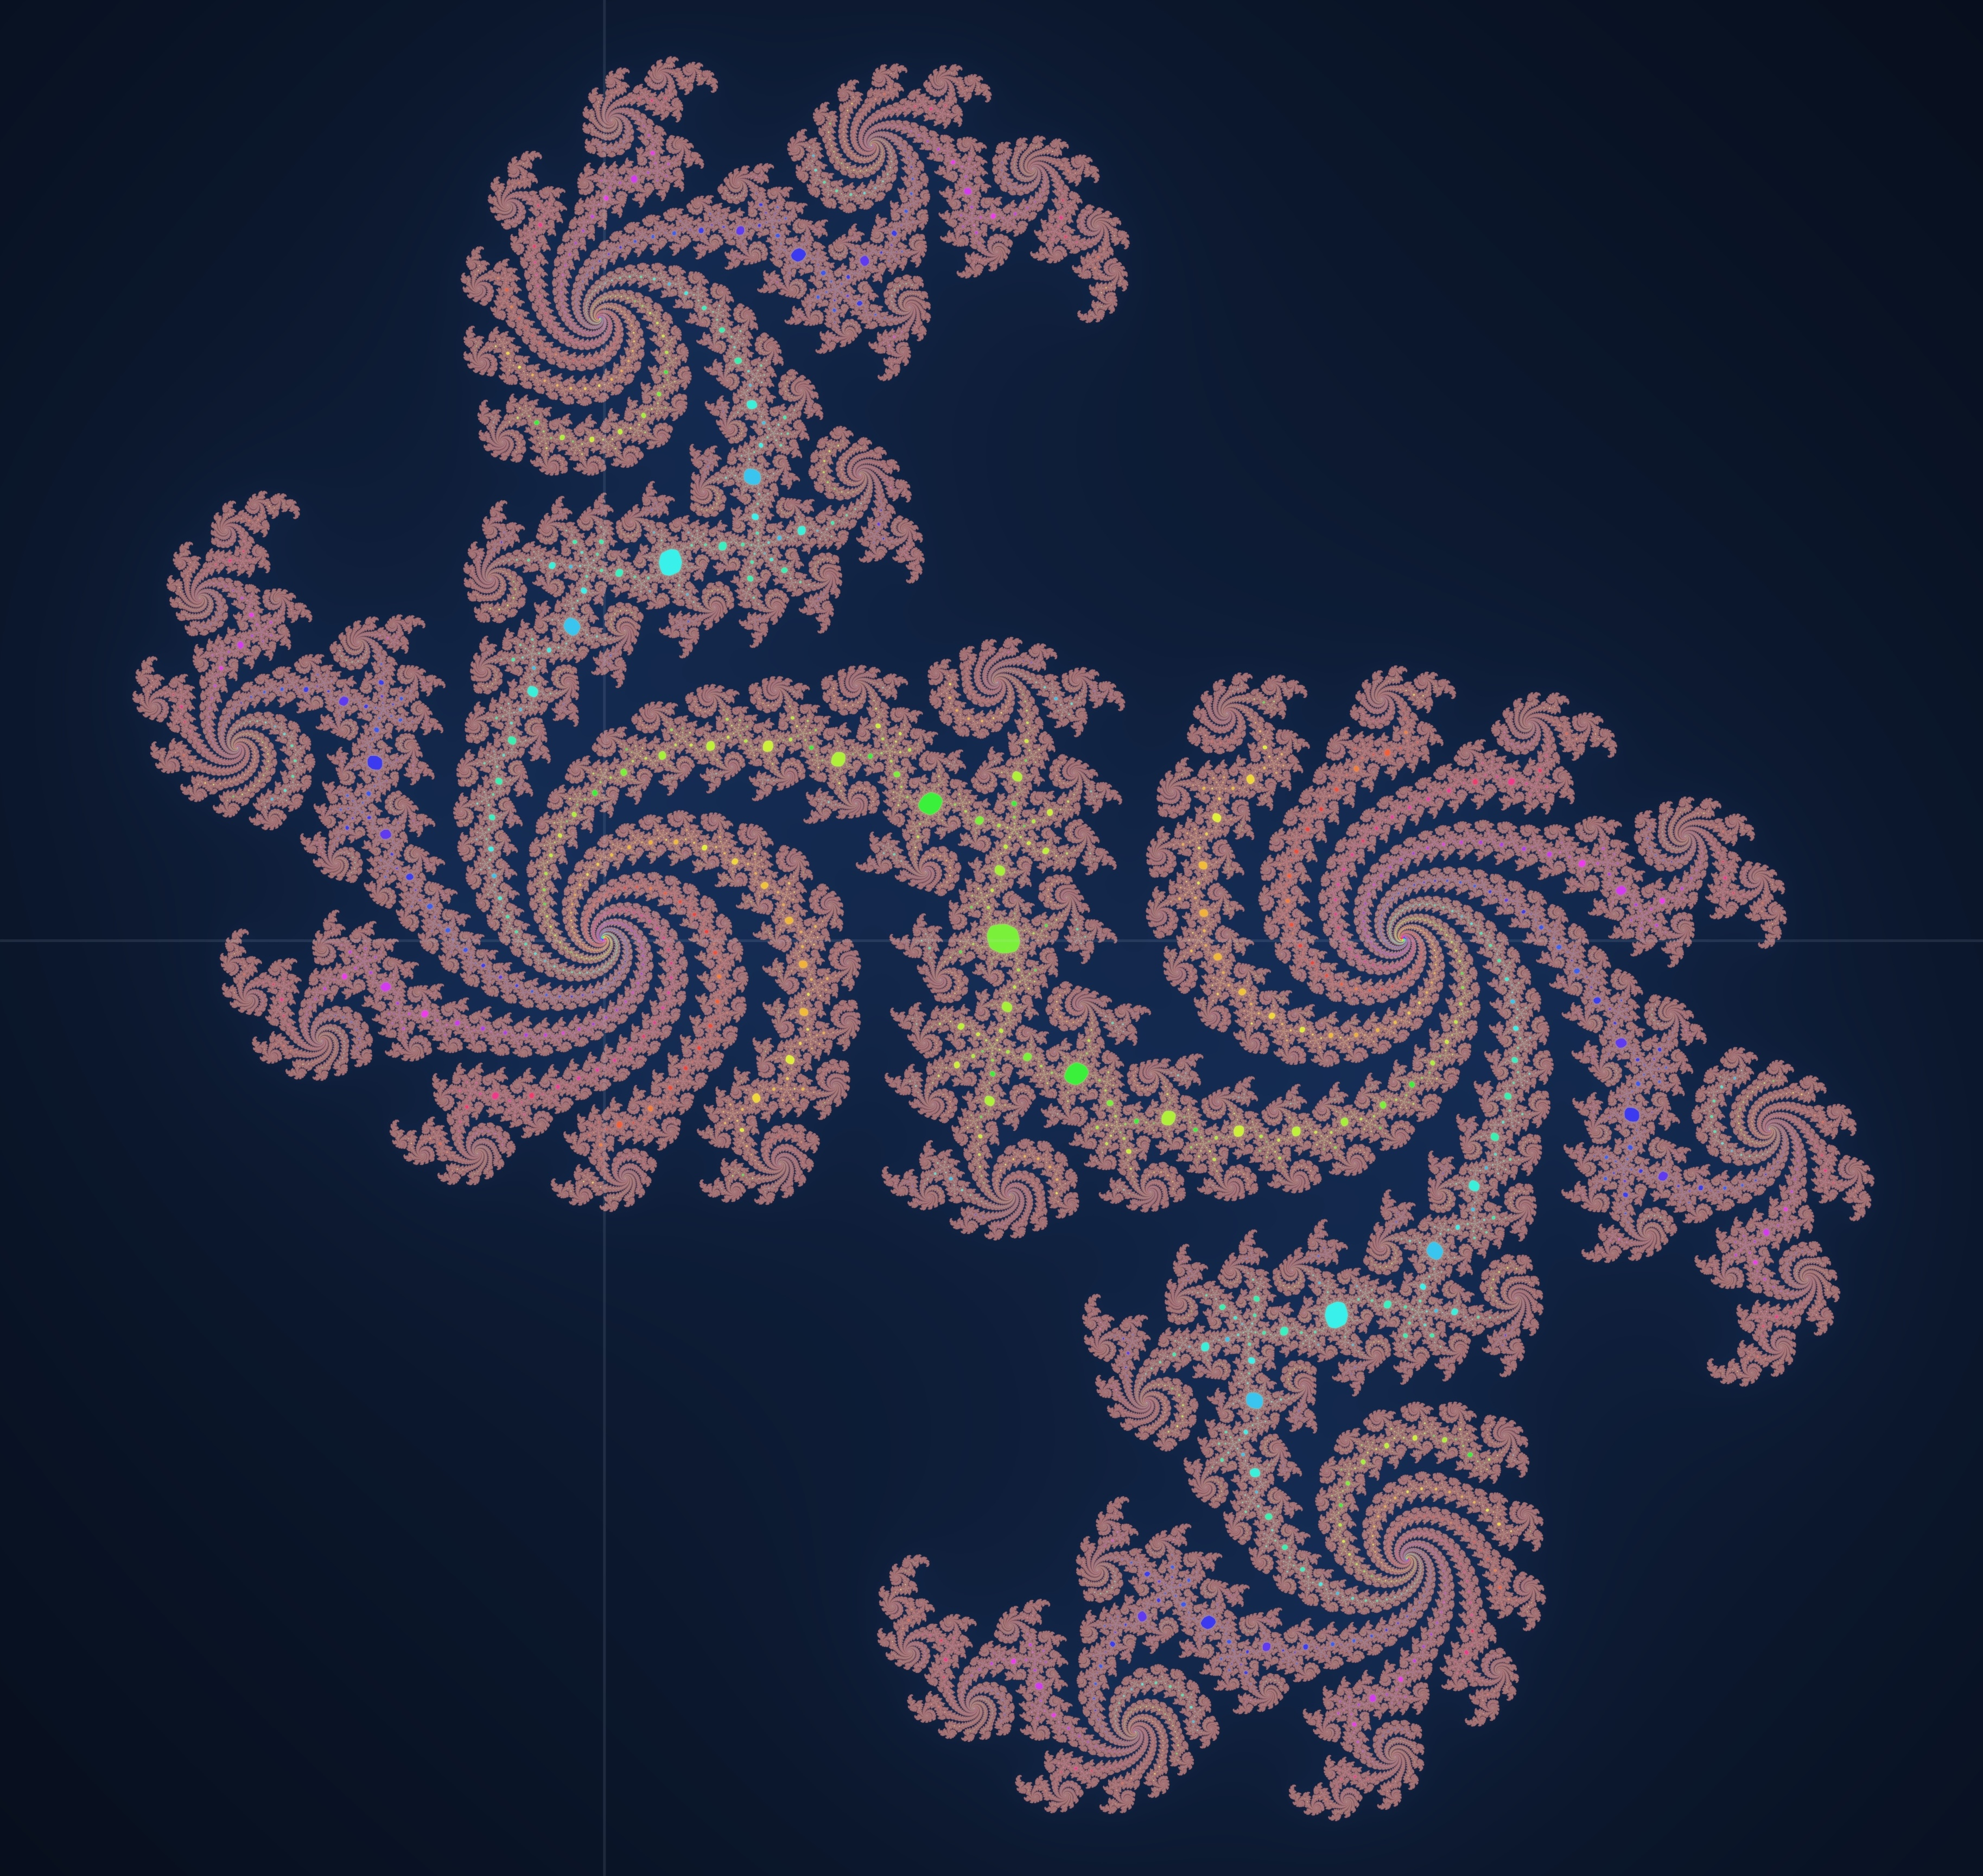
\includegraphics[width=\textwidth]{pictures/newG.jpg}
        \caption{$r=0.614-0.80792i$}
    \end{subfigure}

    \caption{Five deep zooms outside the attracting window, with $|r|$ equal to
    $1.147$, $1.582$, $1.582$, $1.568$ and $1.015$ in panel order. Since all
    exceed one, none shows the attracting Koenigs chart; the images instead
    place the branching segment $r=2p\in(0,1)$ within the wider complex
    quadratic family.}
    \label{fig:koenigs-gallery}
\end{figure}

\FloatBarrier

\subsection{Beyond the attracting window}

Figure~\ref{fig:koenigs-gallery} places the short real interval
$r=2p\in(0,1)$ within the wider complex quadratic family. Every displayed
multiplier has $|r|>1$, so these deep zooms were generated outside the regime of
the attracting Koenigs coordinate developed above. Their role is comparative:
the probabilistic window is only one real segment in a parameter space that
continues in both complex directions. Each image shows only a deep zoom of its
coordinate plate.

\begin{samepage}
The visual complexity makes the negative closed-form result of
Section~\ref{sec:closedform} feel less surprising, but it is not evidence for
the theorem. The result obtained from Becker and Bergweiler concerns the
function $z\mapsto\psi_r(z)$ at each fixed $r$ and is established by the
argument in Appendix~\ref{app:hyper} \cite{BeckerBergweiler1995}; it does not decide whether
the individual number $A(p)$ at any chosen parameter, or the separate map
\[
p\longmapsto A(p)=2\psi_{2p}\!\left(\tfrac12\right)
\]
has a closed form. Nor does a fractal basin boundary by itself preclude a
tractable analytic coordinate: the B\"ottcher coordinate on the basin of infinity
has the same Julia set as boundary and remains explicitly manageable
\cite{Milnor2006}. The pictures provide context for the theorem, not a proof of
it.

The complex-plane view therefore places the scalar $A(p)$ inside the geometry of
the Koenigs coordinate while showing how little of the analytic family the
branching model occupies. That model retains only the real segment
$r=2p\in(0,1)$, ending at the critical boundary $r=1$; on this slice, the
distinguished coordinate value is precisely the survival constant whose
probabilistic consequences were derived above.
\end{samepage}
